\section{実験結果及び考察}
図\ref{fig:CrBuff}にバフ研磨を行った高Cr鋼の表面の撮影結果を示す.ダイヤモンドペーストが3$\mu$mの時にあった黒く長い傷は,1$\mu$mでの研磨によってなくなっている.図\ref{fig:CrEtching}に化学エッチングを行った高Cr鋼の表面の撮影結果を示す.腐食が浅いため分かりにくいが,うっすらと黒い溝がみえる.これが結晶粒界であり,結晶粒の大きさは約50-60$\mu$mであることがわかる.結晶粒界で腐食が進むのは,原子の配列方向が違う隣接する結晶粒をつなぐため,結晶粒界付近の原子の配列方向は乱れており,エネルギー的に不安定であるためである\cite{ミスミ}.全体的に虹色がかかっているように見えるが,これは表面に形成された酸化被膜よる影響と考えられる.

\begin{figure}[htbp]
    \begin{minipage}[htbp]{0.45\linewidth}
      \centering
      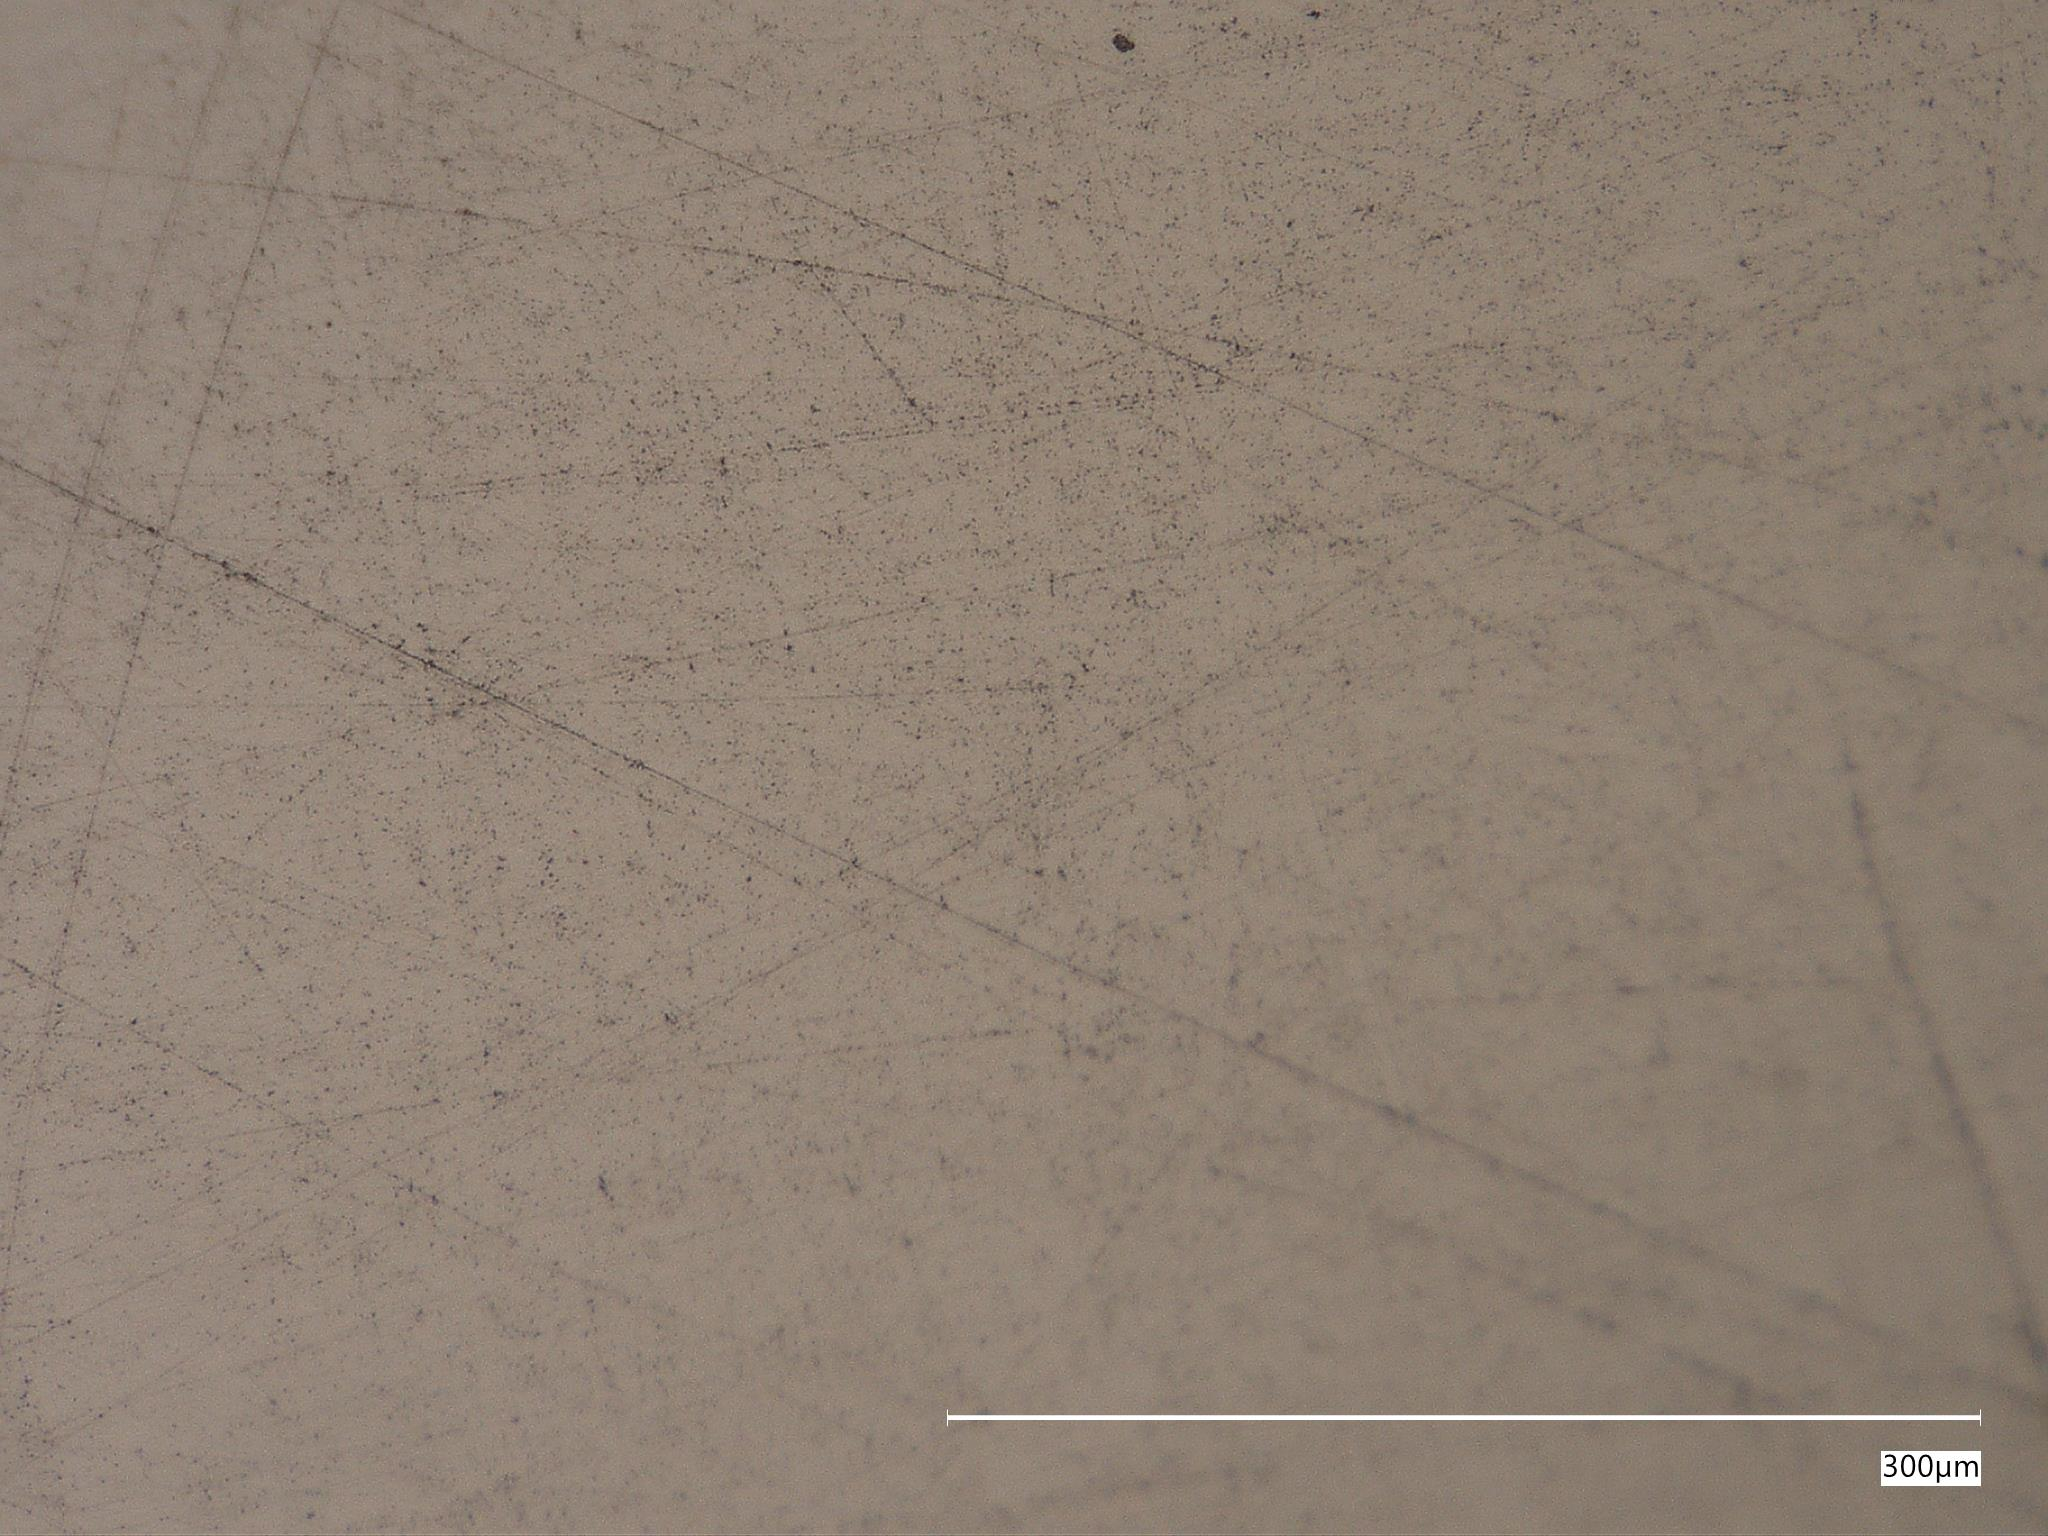
\includegraphics[keepaspectratio, scale=0.07]{fig/241218_9Cr_3um.jpg}
      \subcaption{Diamond paste 3$\mu$m}
      \label{fig:Cr3um}
    \end{minipage}
    \begin{minipage}[htbp]{0.45\linewidth}
      \centering
      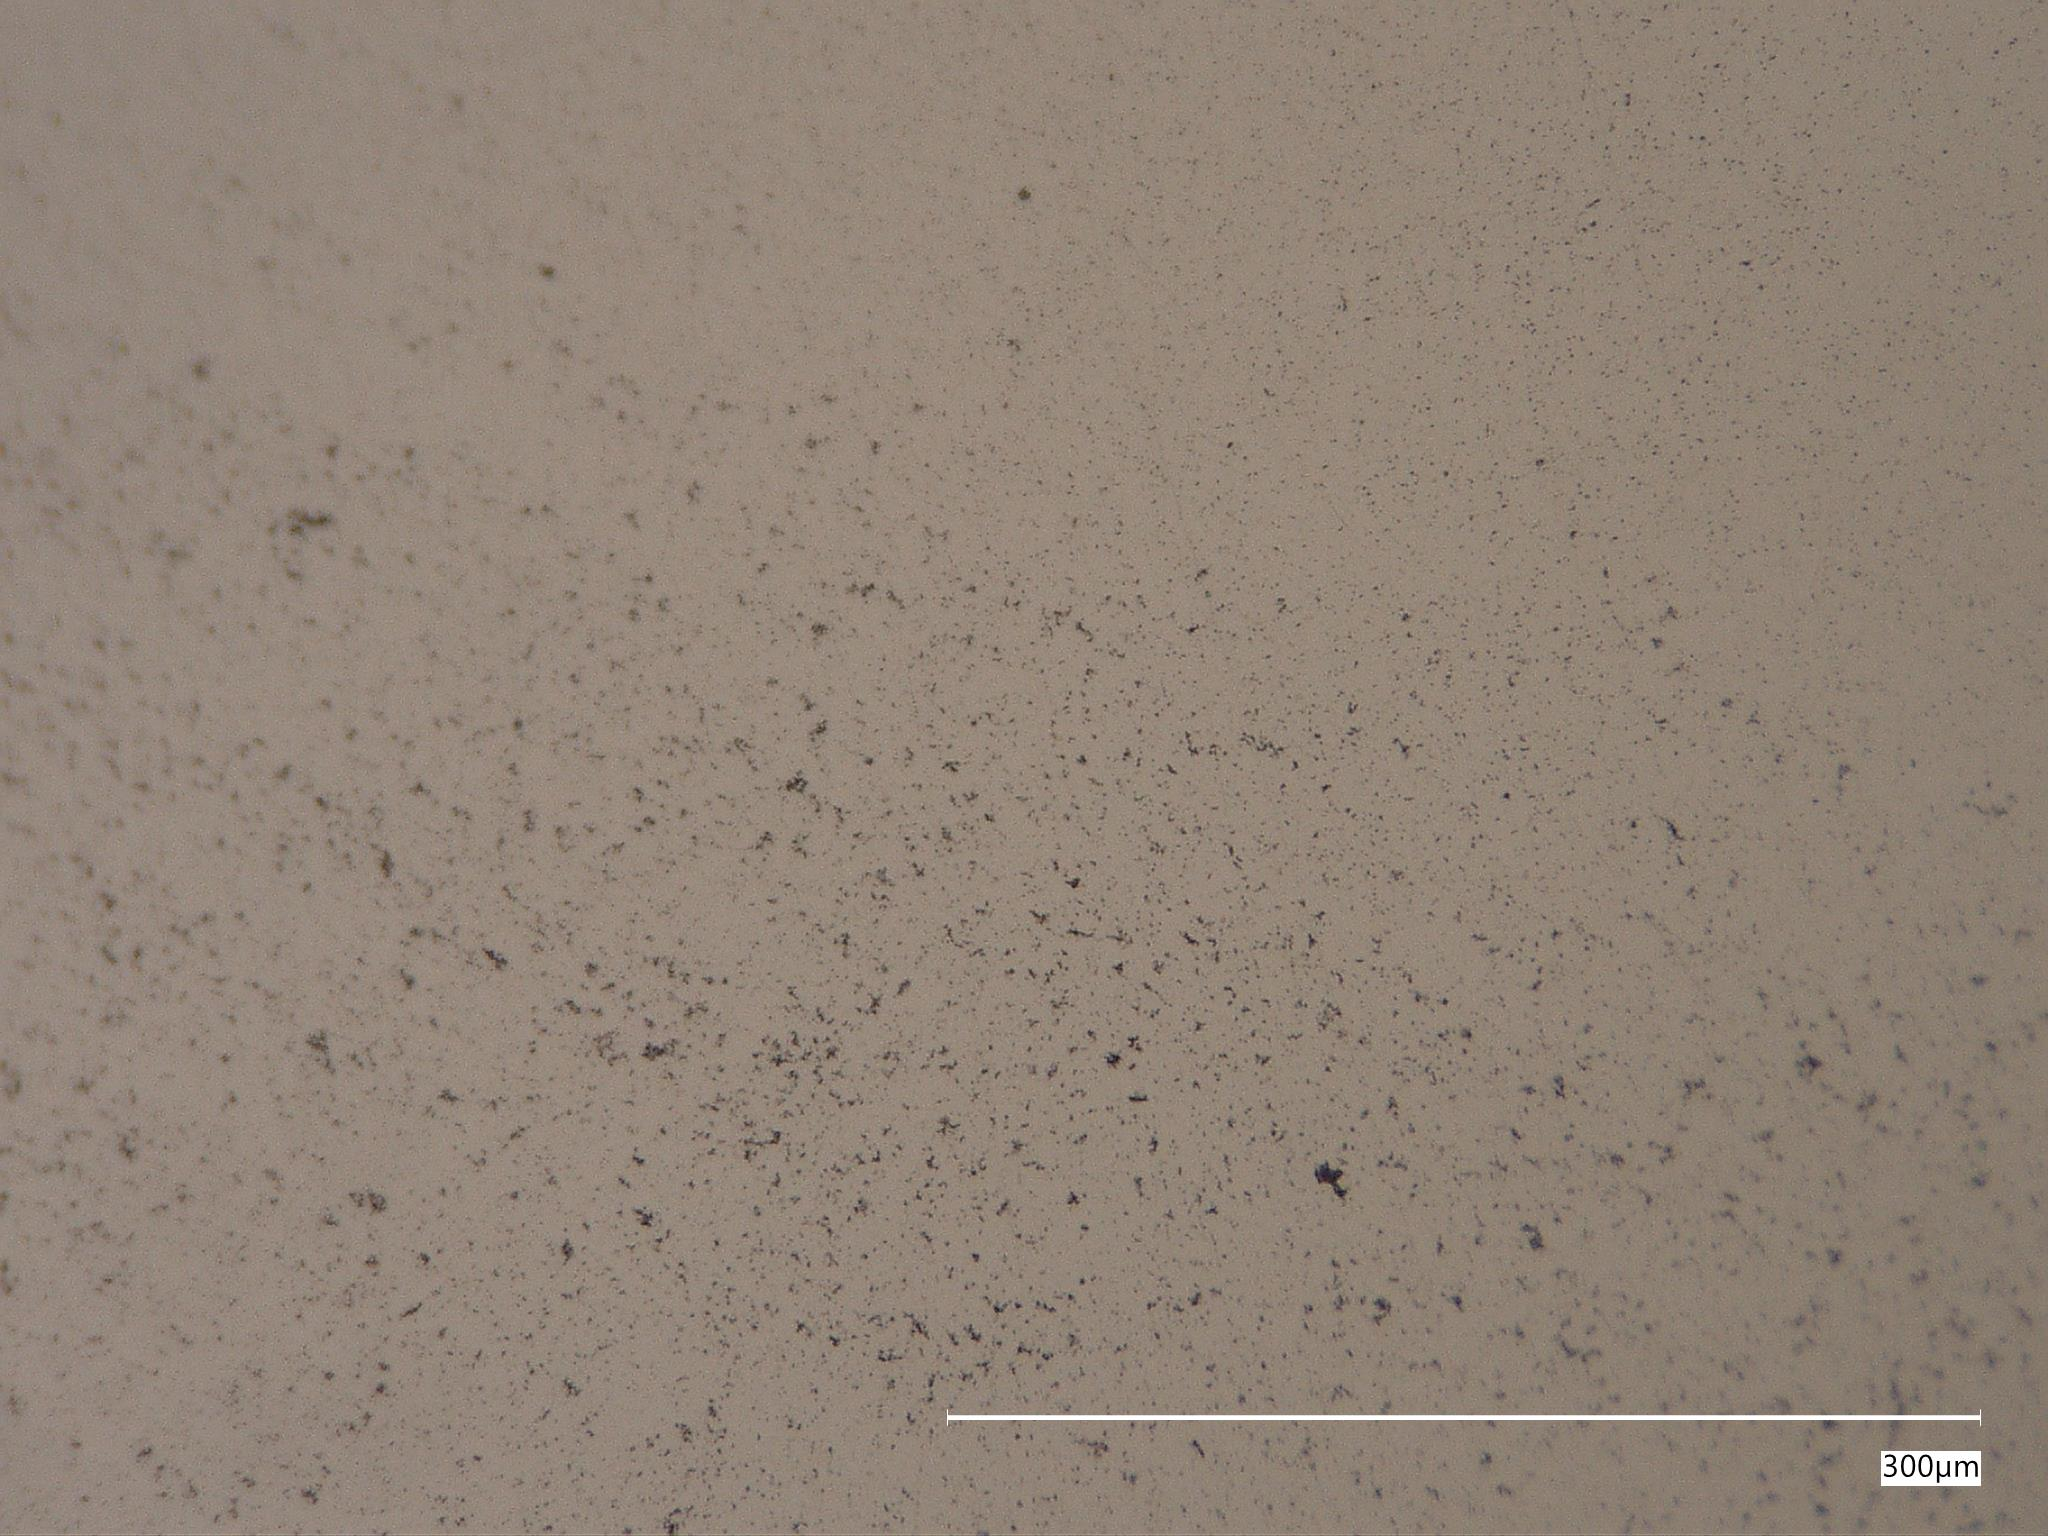
\includegraphics[keepaspectratio, scale=0.07]{fig/241218_9Cr_1um.jpg}
      \subcaption{Diamond paste 1$\mu$m}
      \label{fig:Cr1um}
    \end{minipage}
    \centering
    \caption{High Cr steel after buffing.}
    \label{fig:CrBuff}
\end{figure} 
\clearpage
\begin{figure}[htbp]
    \centering %中央揃え
    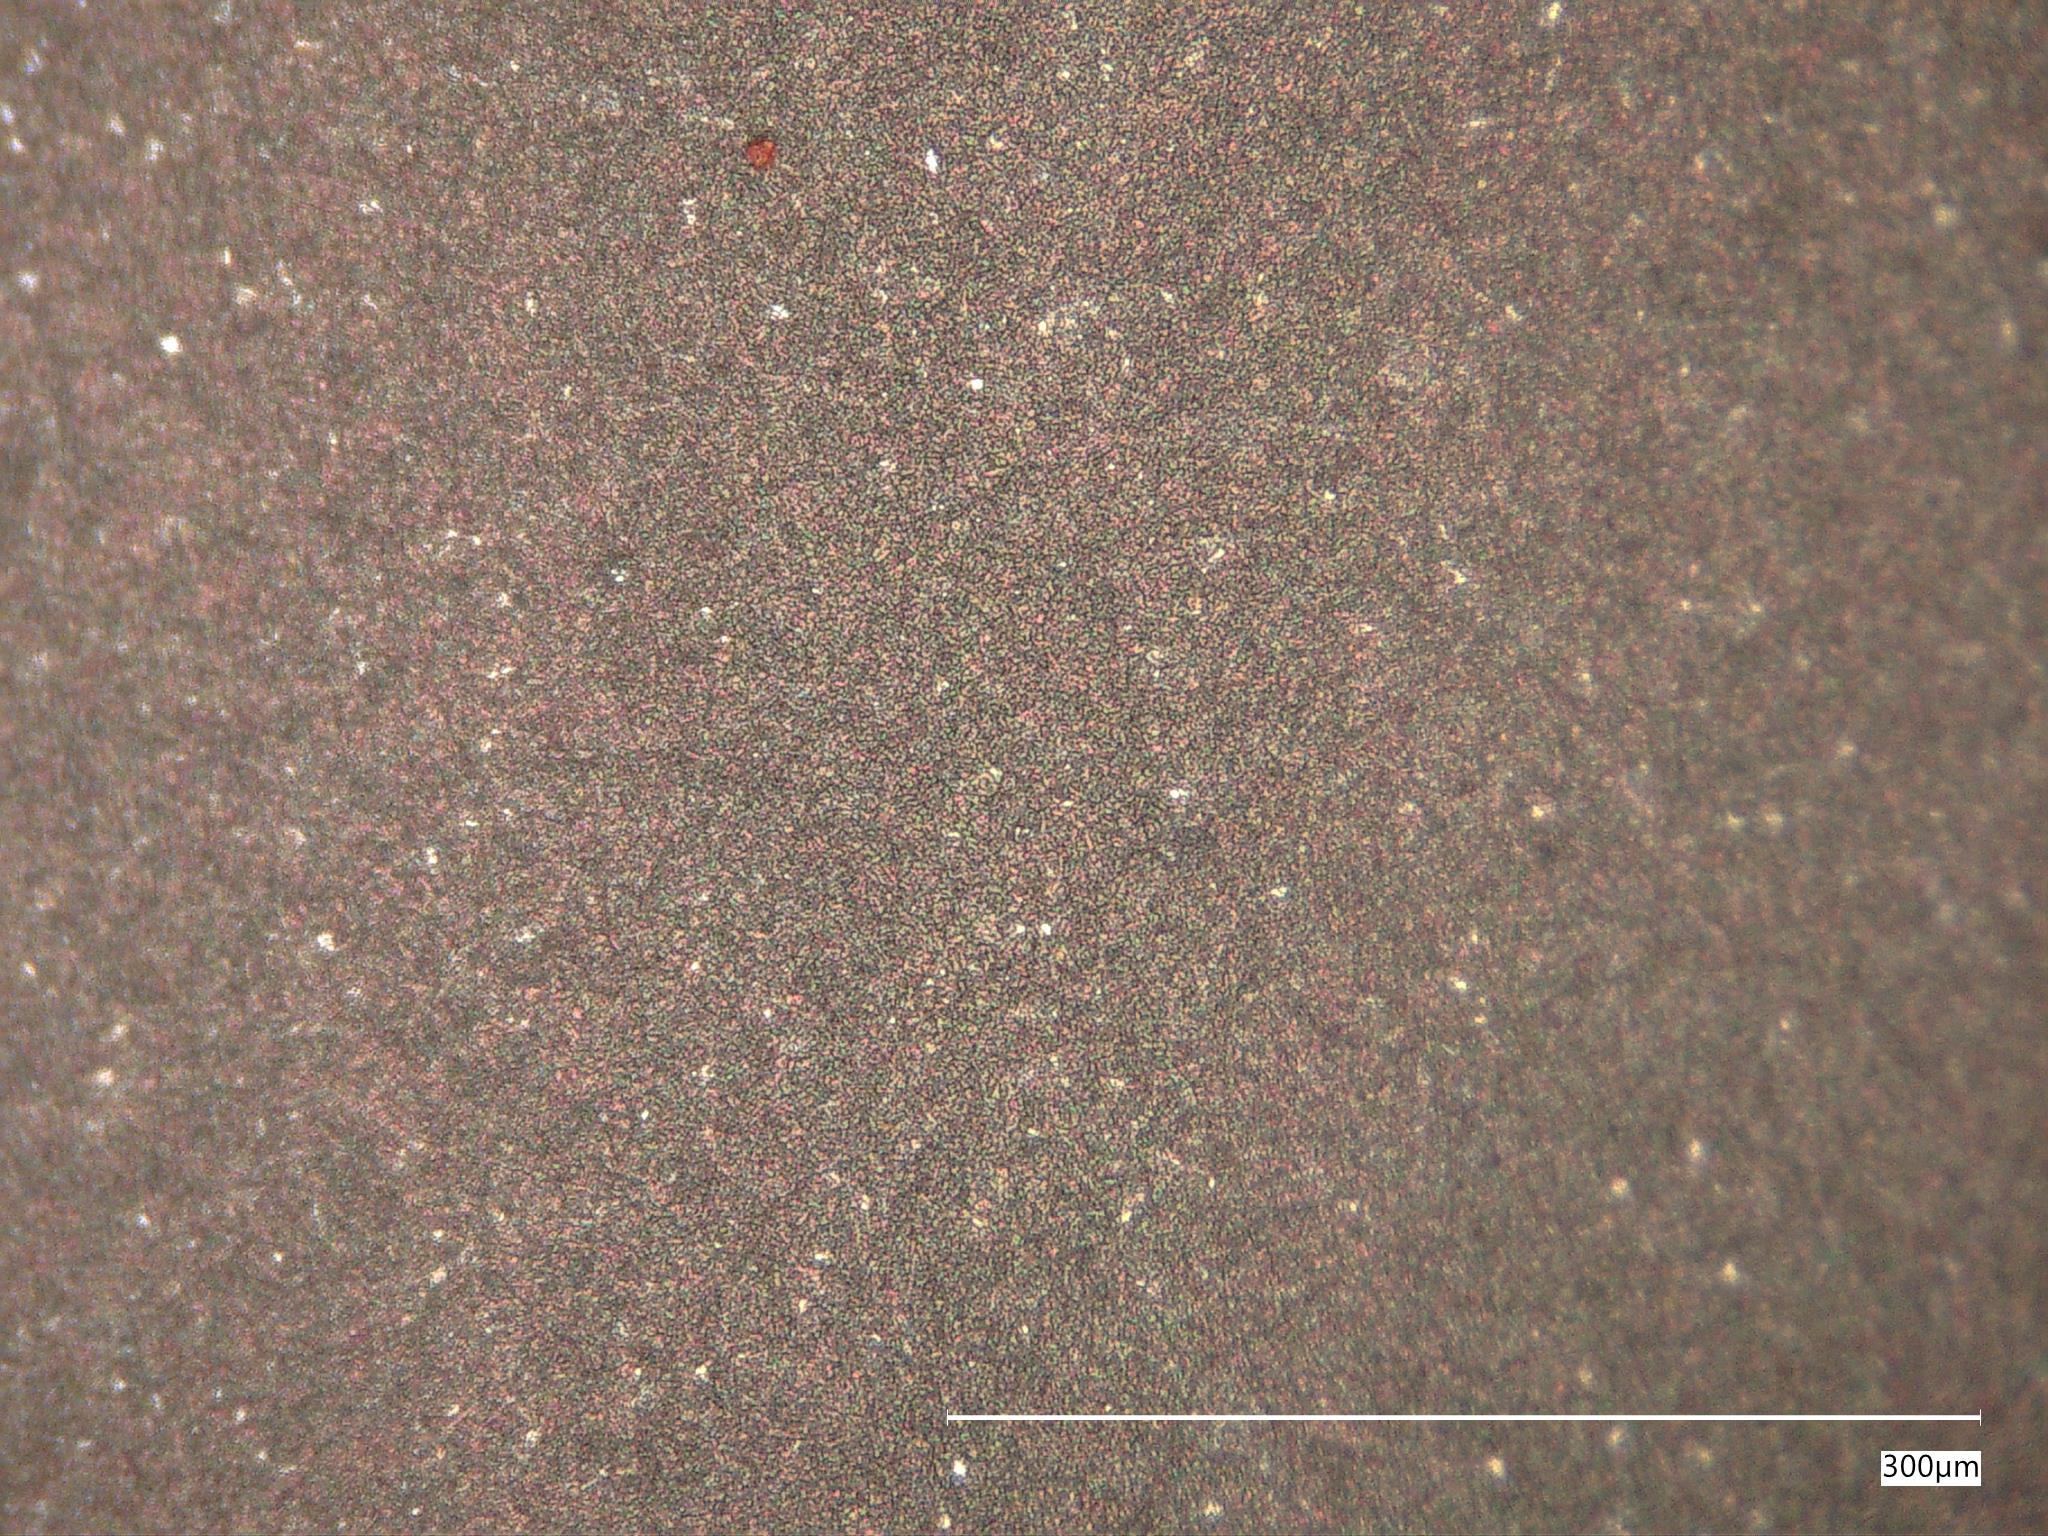
\includegraphics[width=100truemm,clip]{fig/241218_9Cr_etching.jpg}
    \caption{High Cr steel after chemical etching.}
    \label{fig:CrEtching}
\end{figure}

SUS304(MA),SUS304(650$^\circ$C 2hour),SUS304(650$^\circ$C 2hour + 850$^\circ$C 2hour)にバフ研磨を行ったときの表面撮影結果を図\ref{fig:304MABuff},図\ref{fig:304650Buff},図\ref{fig:304850Buff}にそれぞれ示す.それぞれにおいて,高Cr鋼のときと同様にダイヤモンドペーストが3$\mu$mの時にあった黒く長い傷は,1$\mu$mでの研磨によってなくなっている.SUS304(MA),SUS304(650$^\circ$C 2hour),SUS304(650$^\circ$C 2hour + 850$^\circ$C 2hour)に電気化学エッチングを行ったときの表面撮影結果を図\ref{fig:304MAEtching},図\ref{fig:304650Etching},図\ref{fig:304850Etching}にそれぞれ示す.SUS304(MA)の場合,全体的に薄っすらと腐食されており,ややへこんだ結晶粒が黒っぽくなっている.SUS304(650$^\circ$C 2hour)の場合,結晶粒界が強く腐食されており,結晶粒がくっきり現れている.SUS304(650$^\circ$C 2hour + 850$^\circ$C 2hour)の場合も結晶粒界が黒く腐食されているが,SUS304(650$^\circ$C 2hour)よりも結晶粒界の線が細く,腐食されやすさが改善していることが分かる.

このような熱処理による腐食しやすさの変化は課題で述べる鋭敏化によるものだと考えられる.650$^\circ$C 2hourの熱処理では,図\ref{fig:鋭敏化}における鋭敏化域にあるため腐食されやすくなり,650$^\circ$C 2hour + 850$^\circ$C 2hourの熱処理では,鋭敏化域を抜け出したため腐食されやすさが改善されたと考えることができる.図\ref{fig:304650Etching},図\ref{fig:304850Etching}では結晶粒界のほかに黒く長い腐食が目立つが,これは元々残っていた細かい傷や,材料内の残留応力によって被膜が破れ腐食しやすい領域が生じたためではないかと考察する.
\begin{figure}[htbp]
    \begin{minipage}[htbp]{0.45\linewidth}
      \centering
      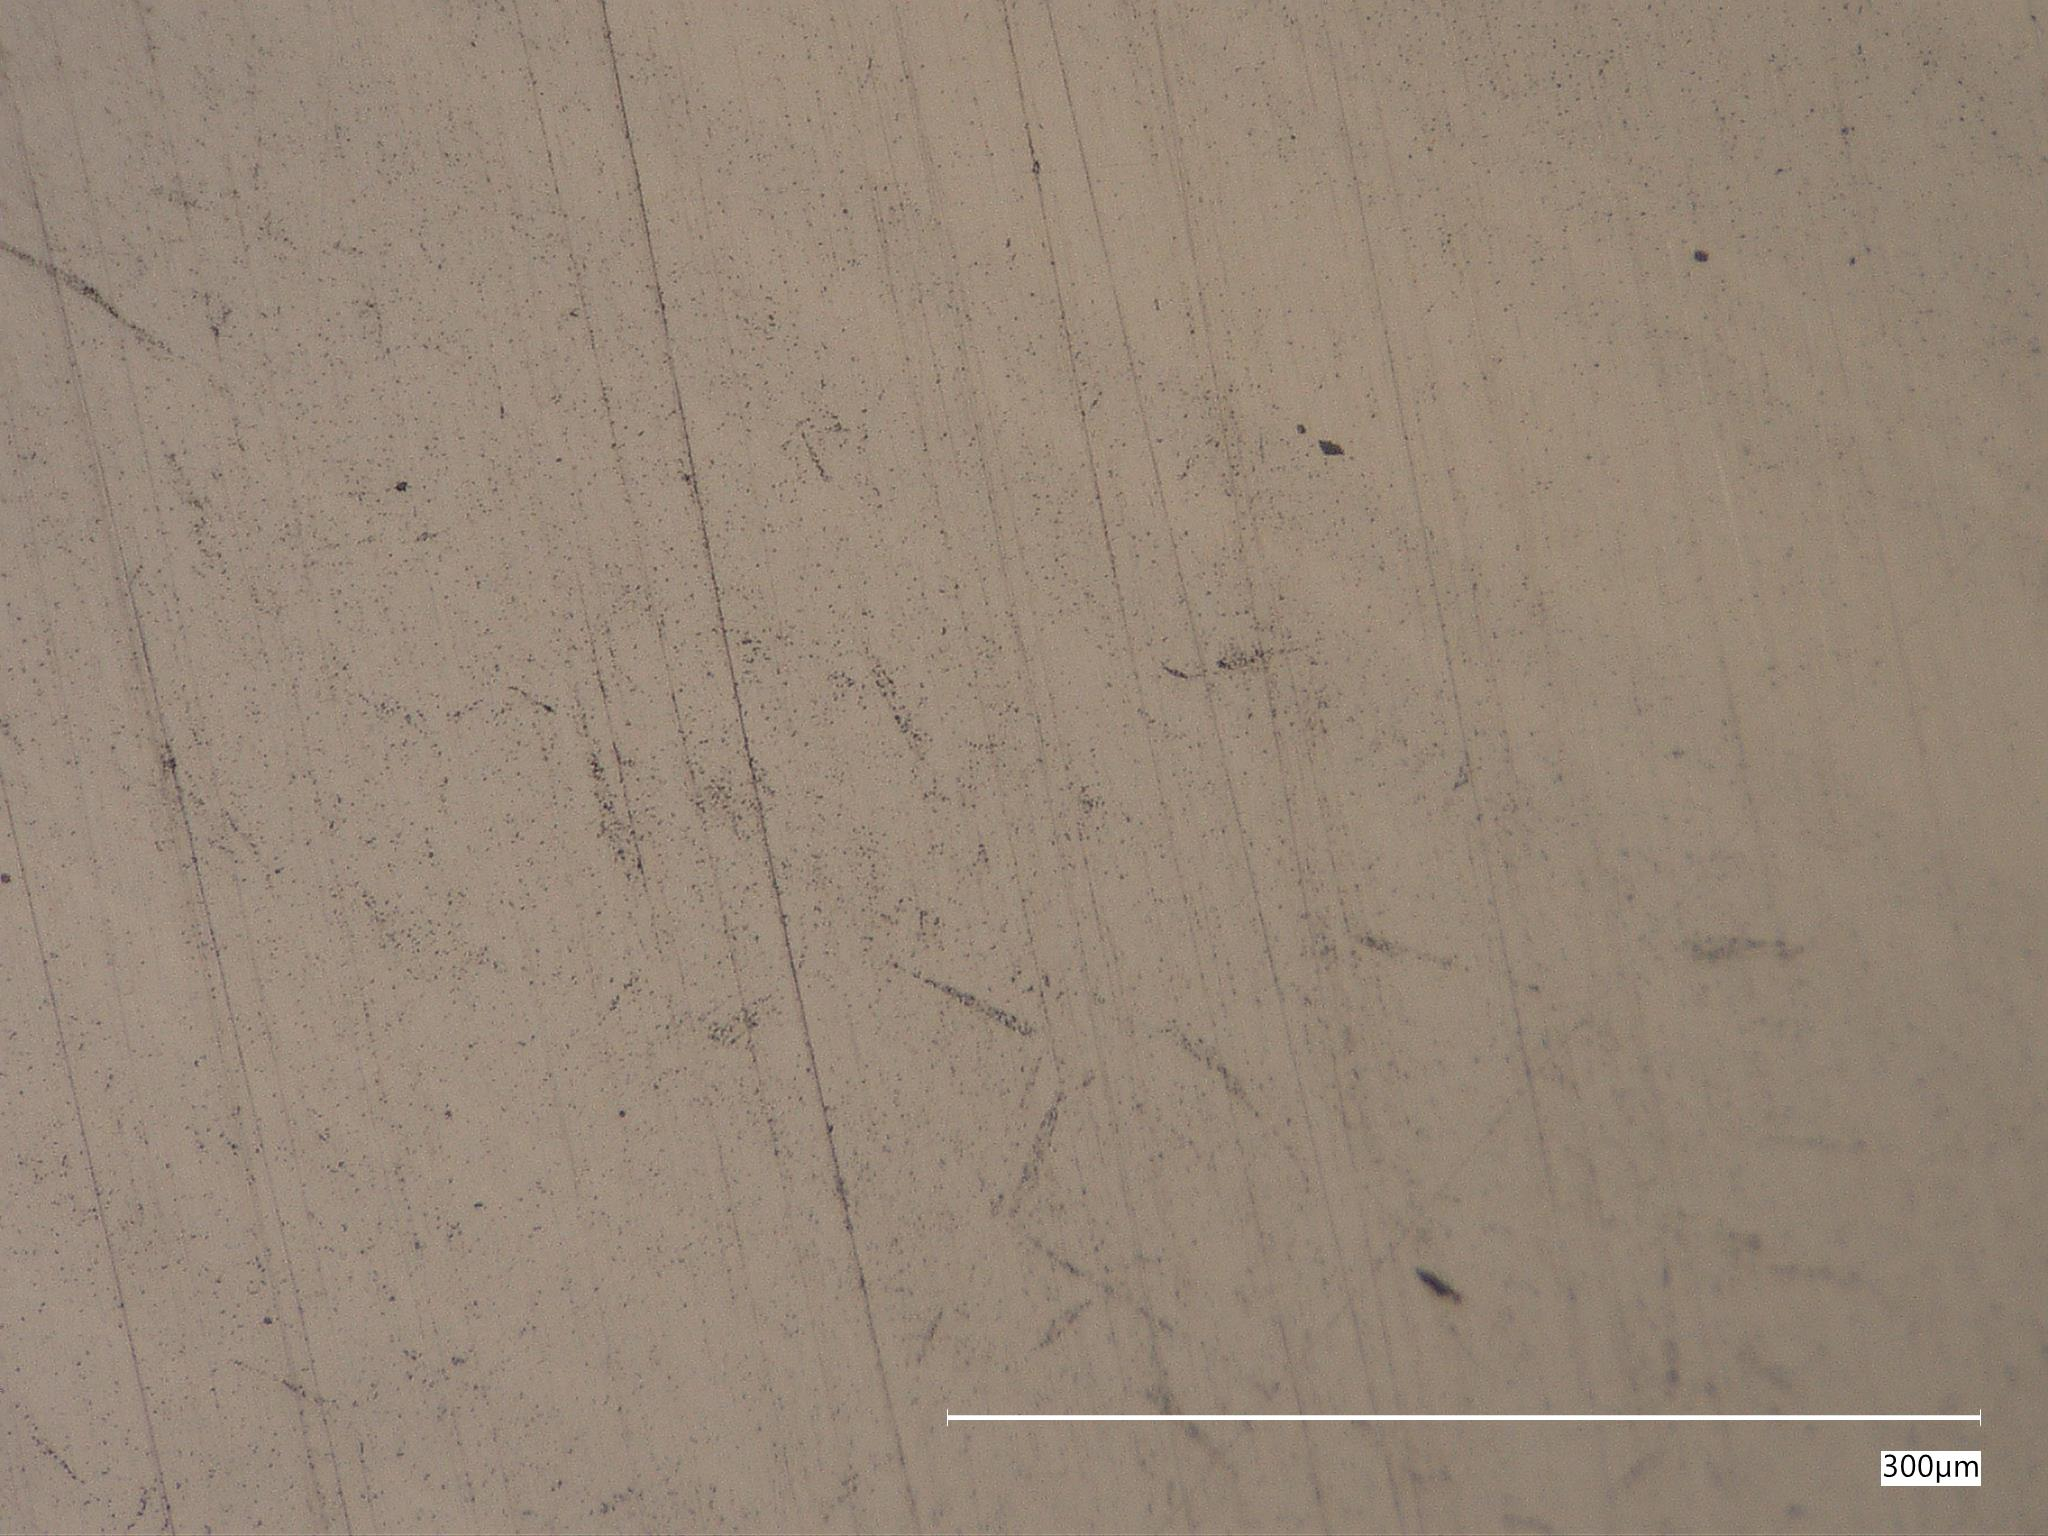
\includegraphics[keepaspectratio, scale=0.07]{fig/241218_304MA_3um.jpg}
      \subcaption{Diamond paste 3$\mu$m}
      \label{fig:MA3um}
    \end{minipage}
    \begin{minipage}[htbp]{0.45\linewidth}
      \centering
      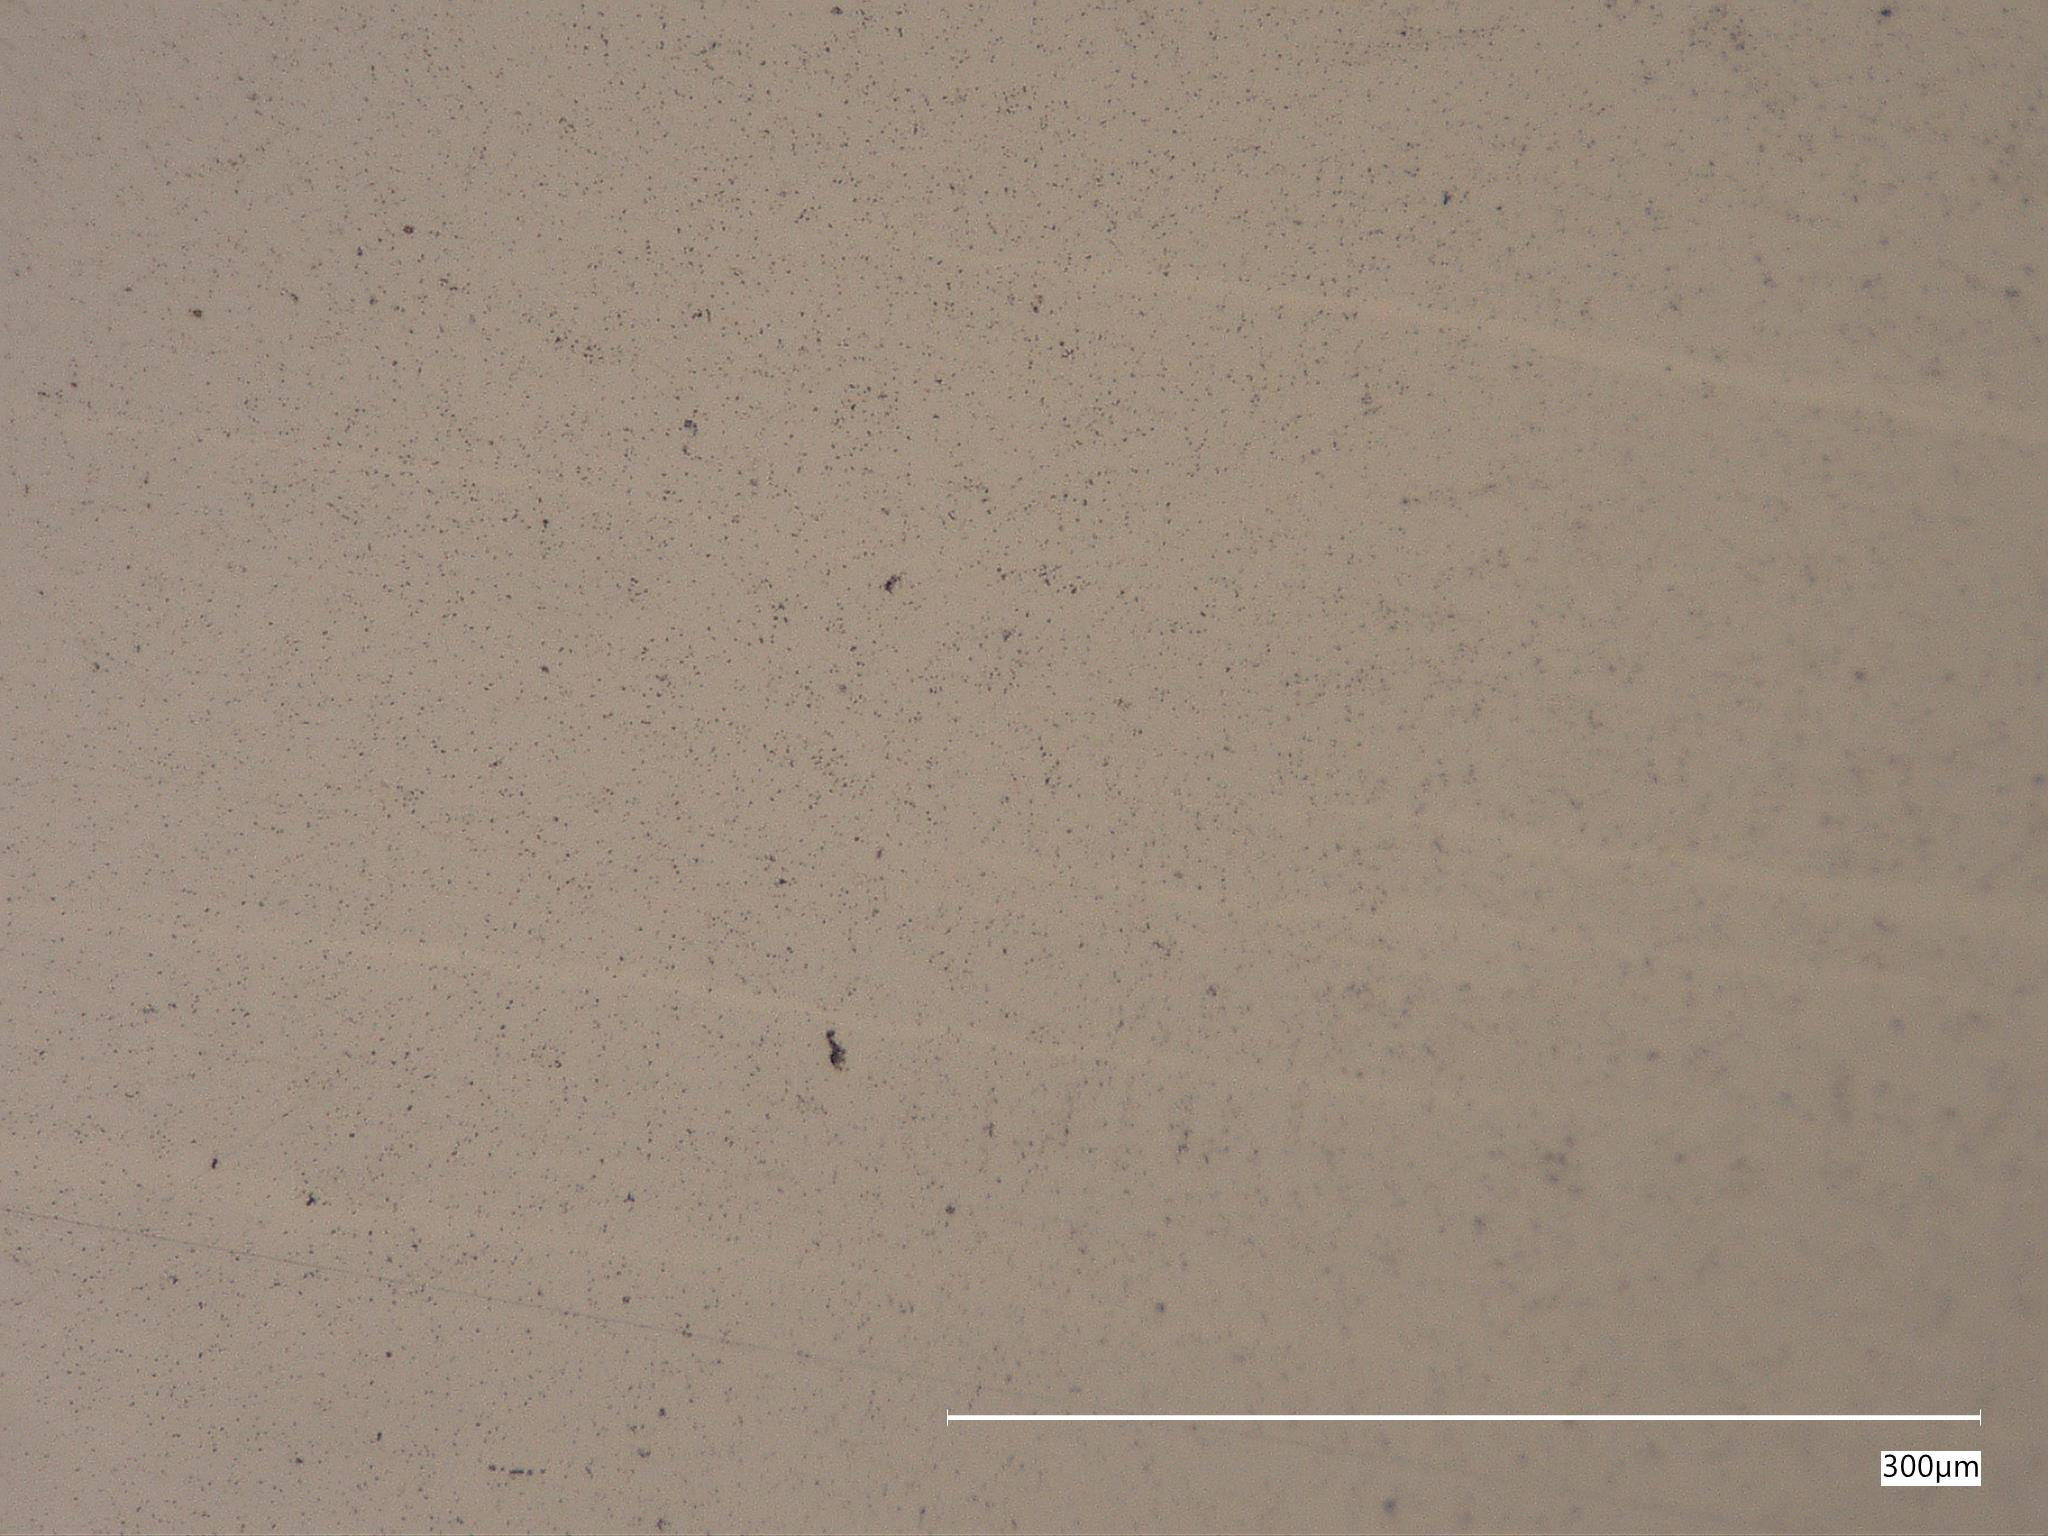
\includegraphics[keepaspectratio, scale=0.07]{fig/241218_304MA_1um.jpg}
      \subcaption{Diamond paste 1$\mu$m}
      \label{fig:MA1um}
    \end{minipage}
    \centering
    \caption{SUS304 stainless steel after buffing(MA).}
    \label{fig:304MABuff}
\end{figure}
\begin{figure}[htbp]
    \centering %中央揃え
    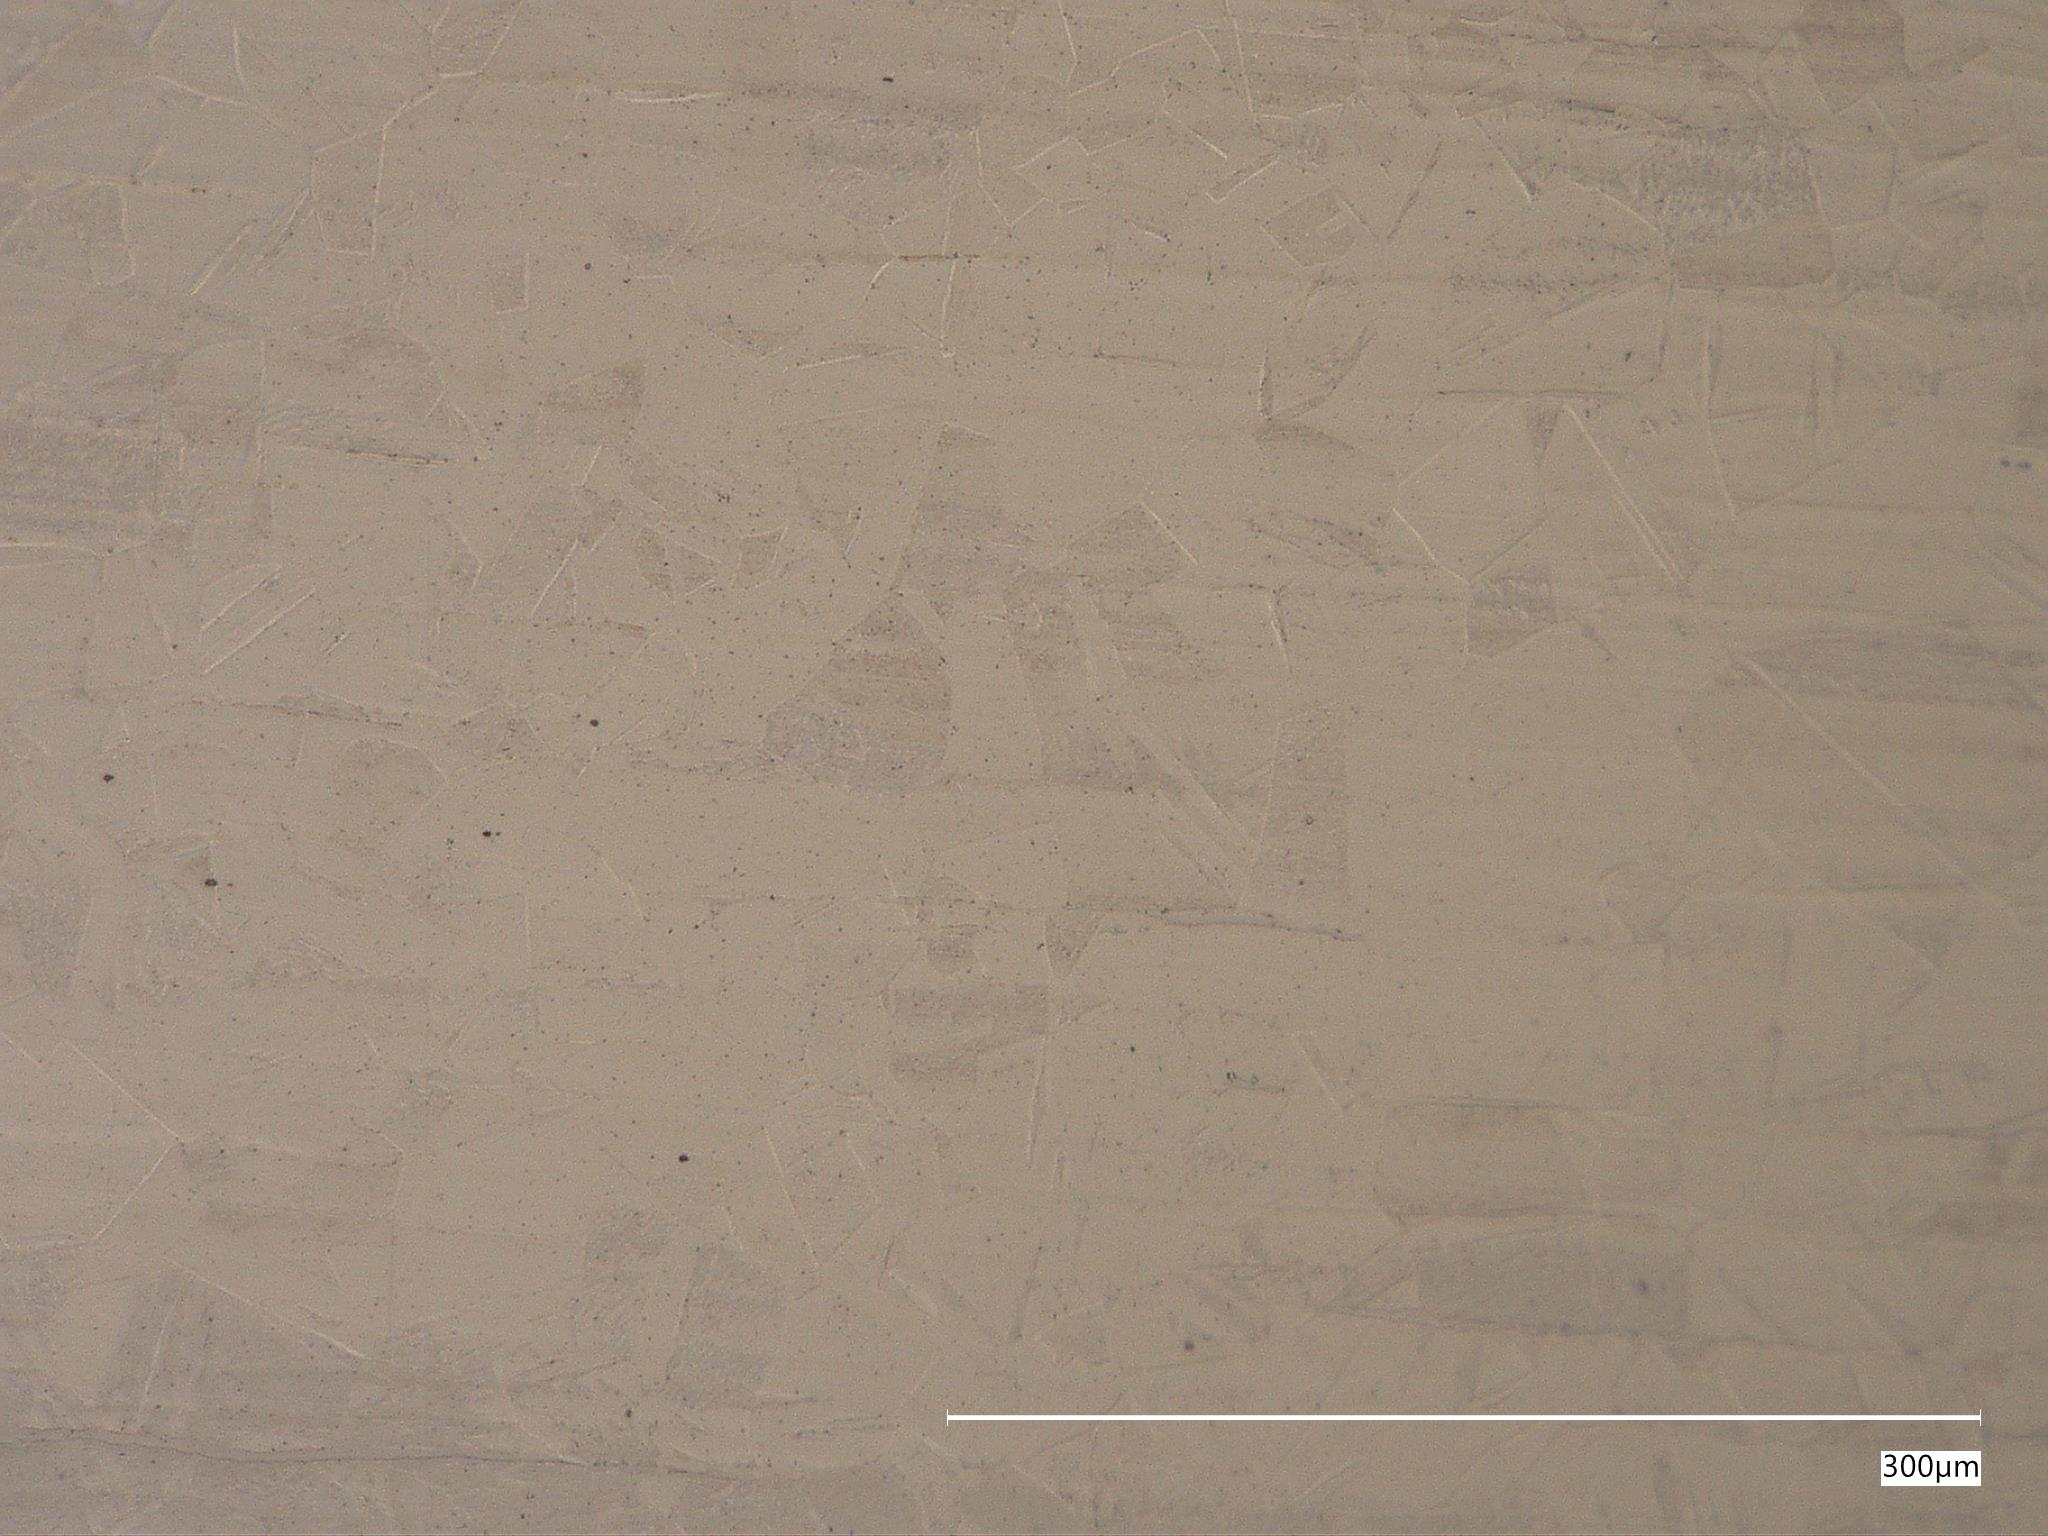
\includegraphics[width=100truemm,clip]{fig/241218_304MA_etching.jpg}
    \caption{SUS304 stainless steel after chemical etching(MA).}
    \label{fig:304MAEtching}
\end{figure}

\begin{figure}[htbp]
    \begin{minipage}[htbp]{0.45\linewidth}
      \centering
      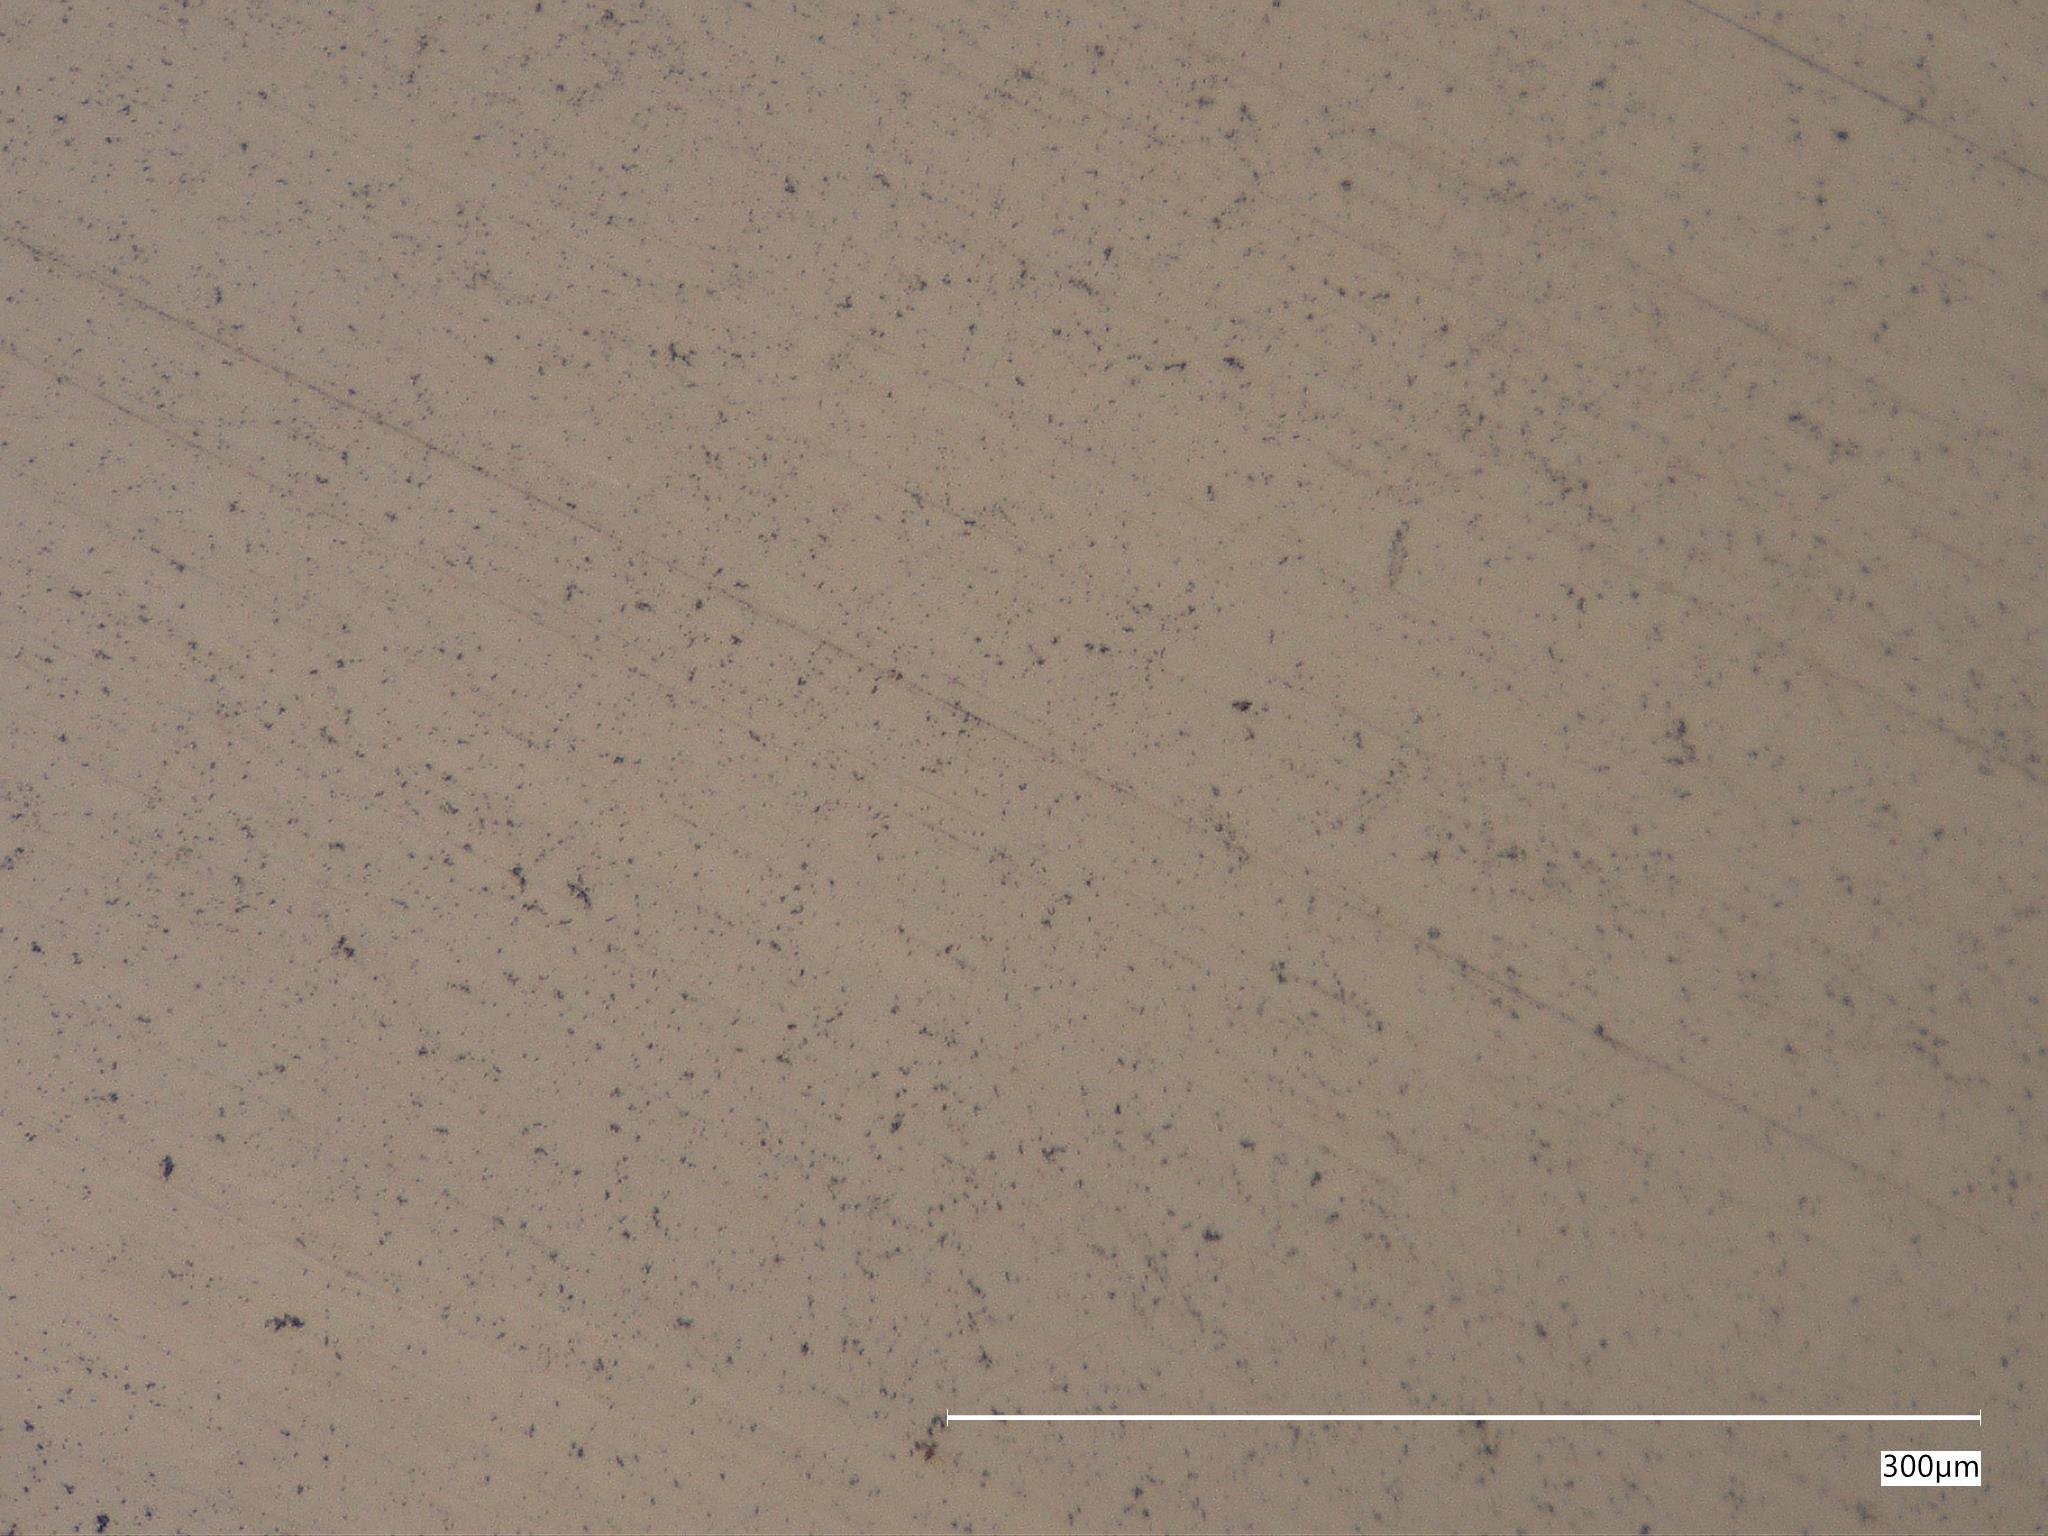
\includegraphics[keepaspectratio, scale=0.07]{fig/241218_304650C2h_3um.jpg}
      \subcaption{Diamond paste 3$\mu$m}
      \label{fig:6503um}
    \end{minipage}
    \begin{minipage}[htbp]{0.45\linewidth}
      \centering
      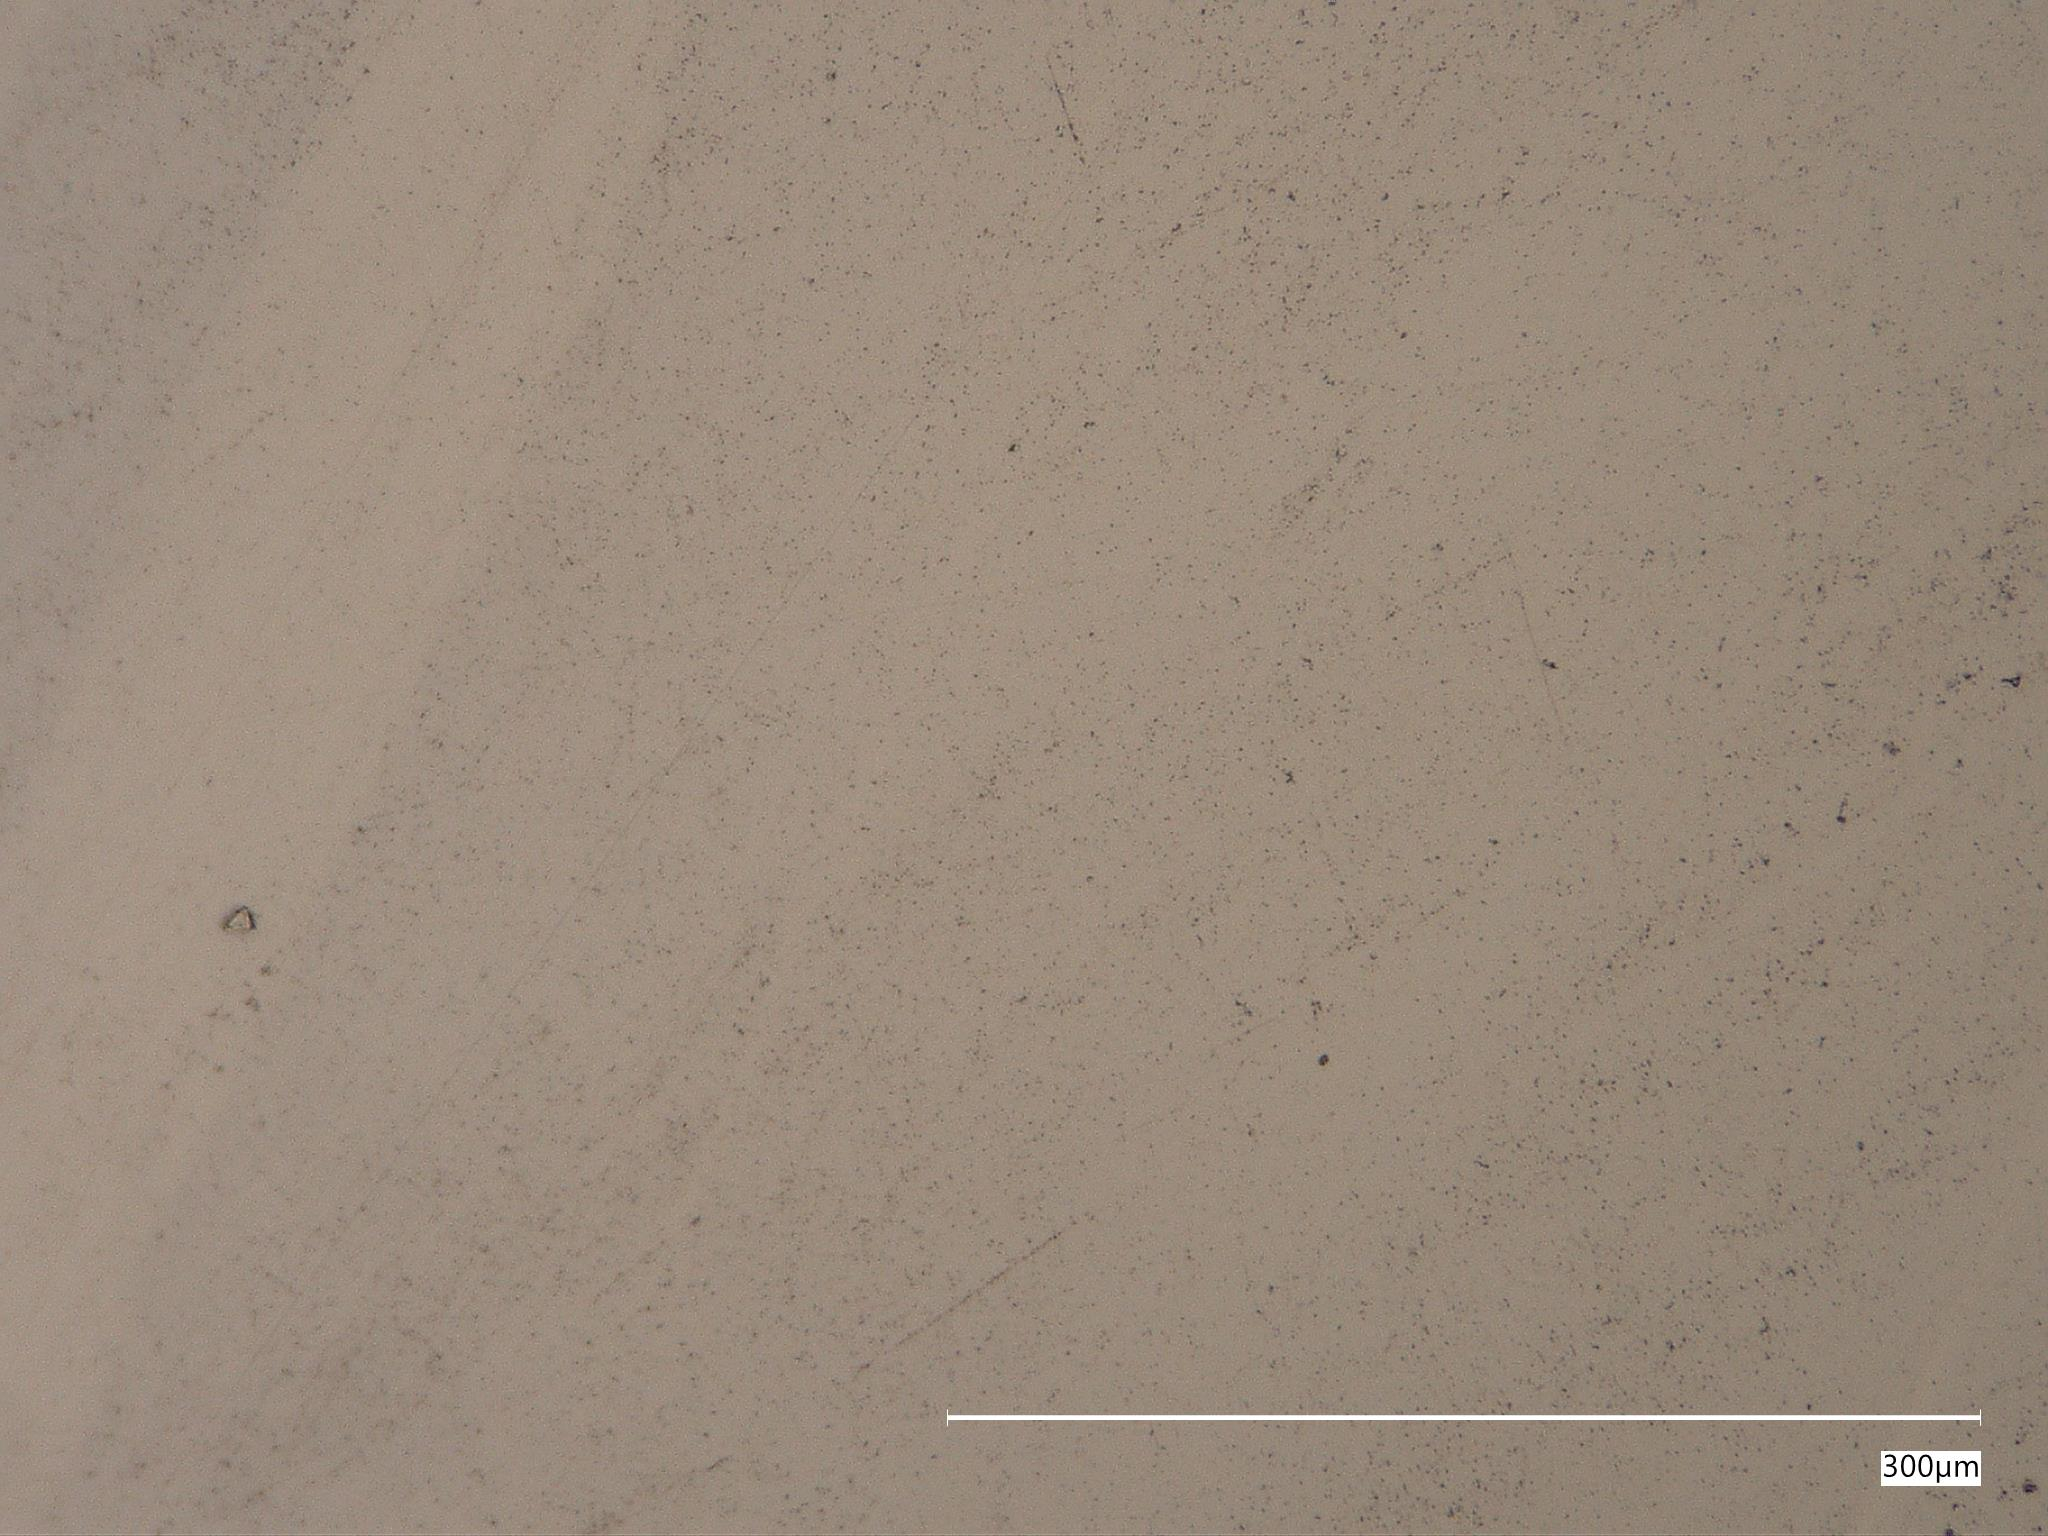
\includegraphics[keepaspectratio, scale=0.07]{fig/241218_304650C2h_1um.jpg}
      \subcaption{Diamond paste 1$\mu$m}
      \label{fig:6501um}
    \end{minipage}
    \centering
    \caption{SUS304 stainless steel after buffing(650$^\circ$C 2hour).}
    \label{fig:304650Buff}
\end{figure}
\begin{figure}[htbp]
    \centering %中央揃え
    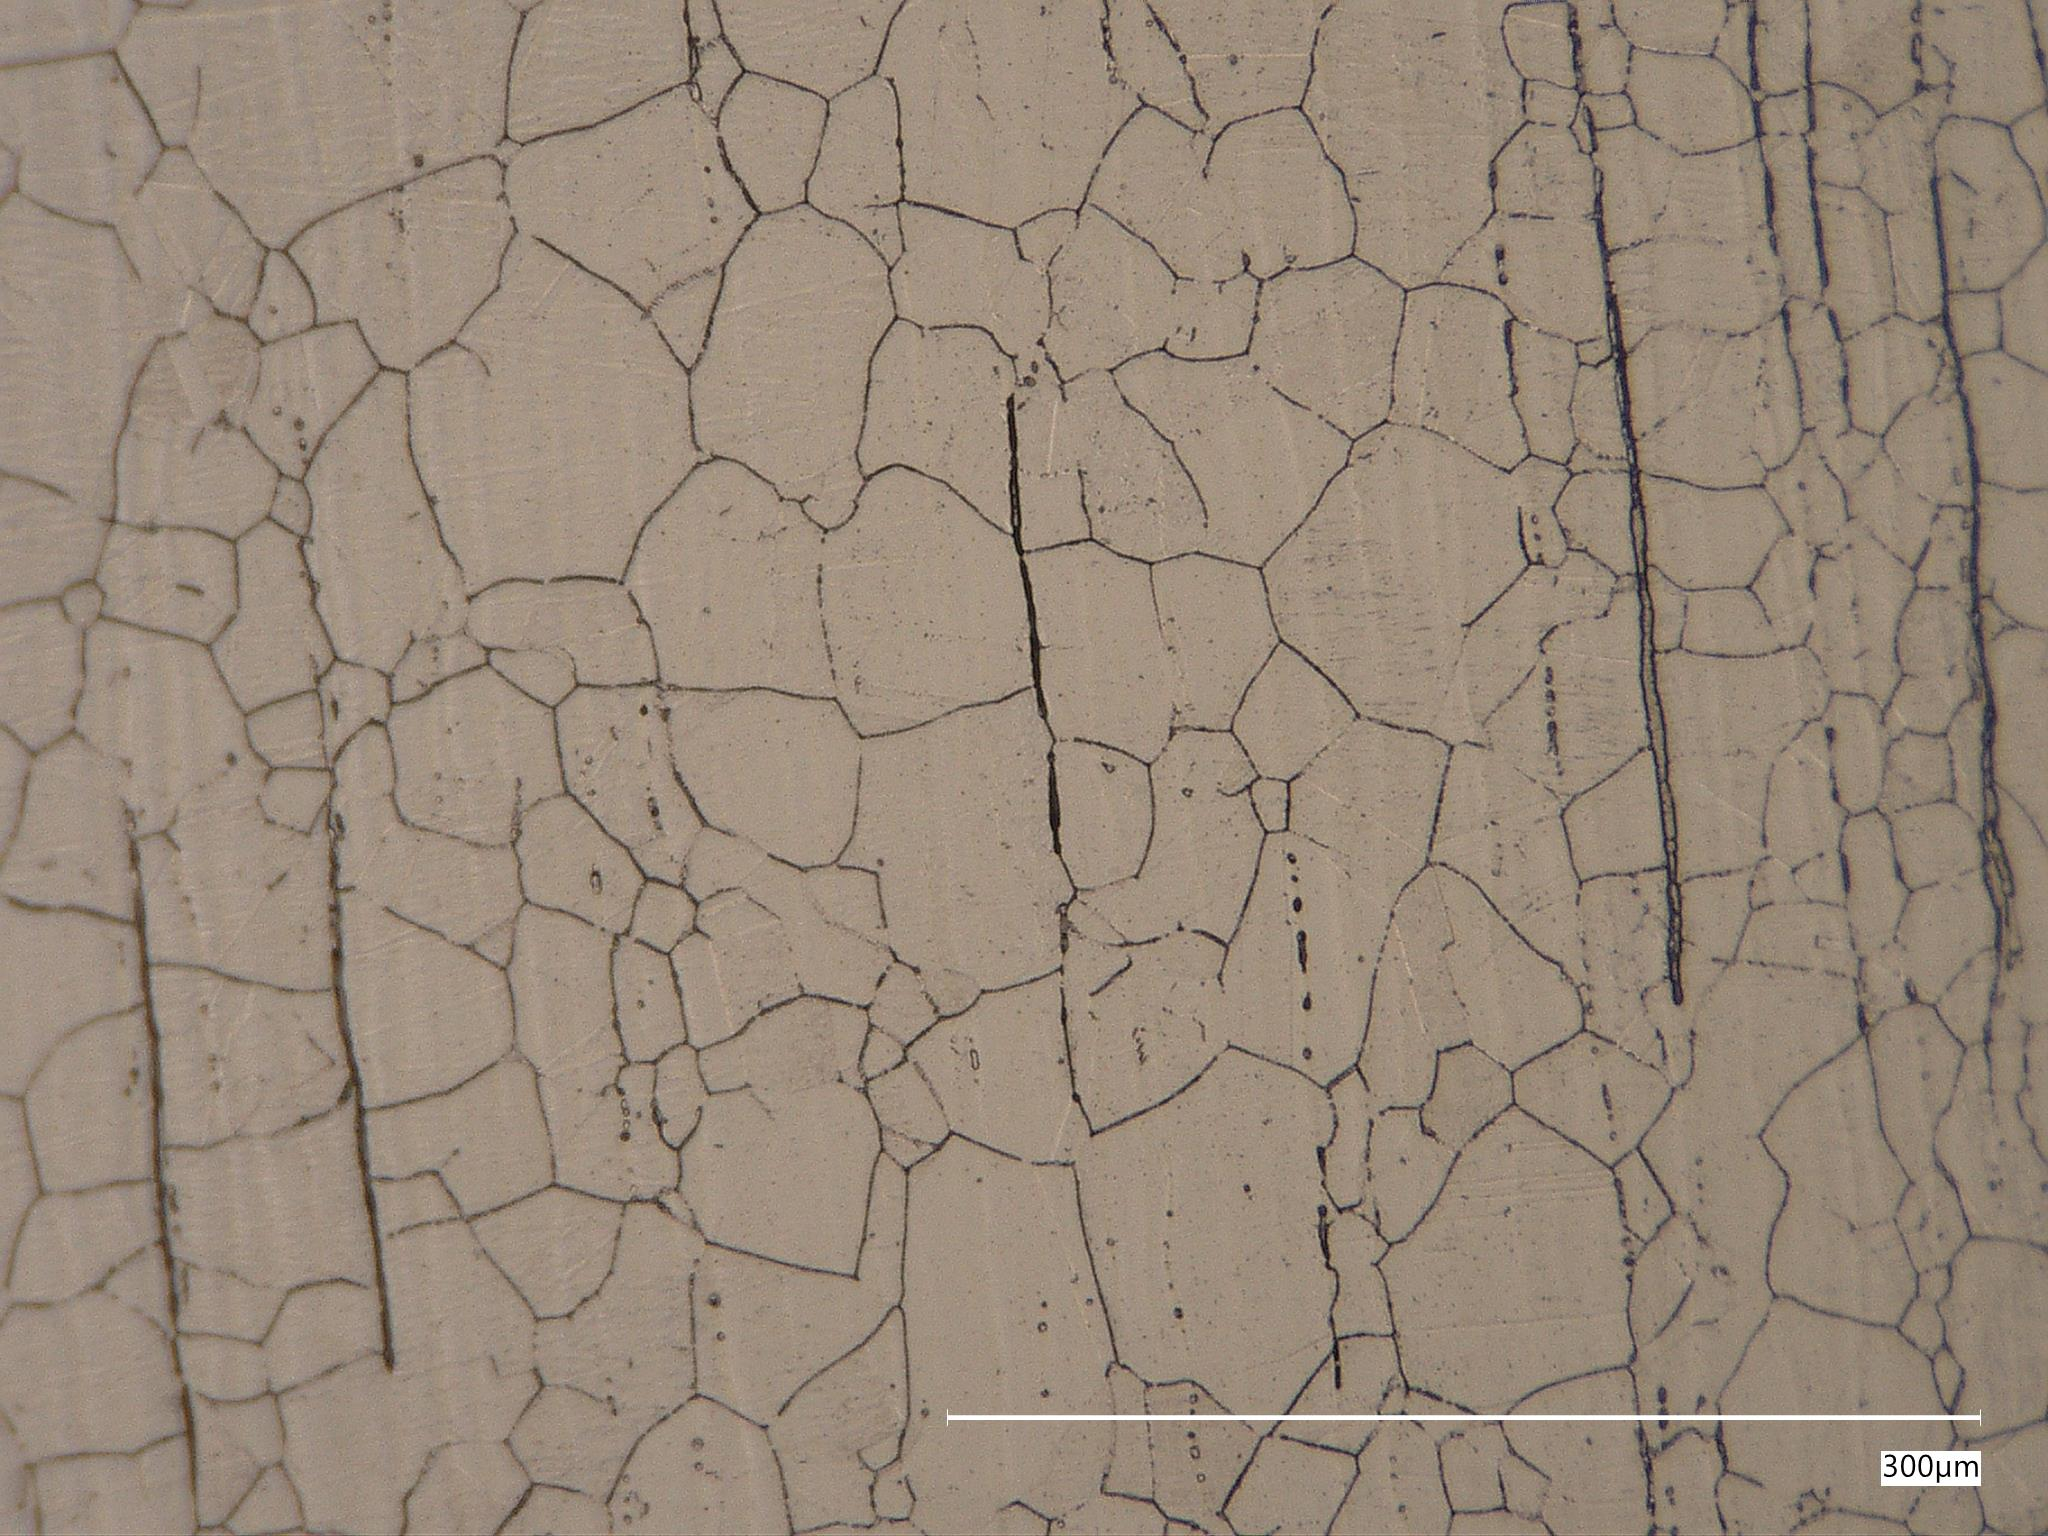
\includegraphics[width=100truemm,clip]{fig/241218_304650C2h_etching.jpg}
    \caption{SUS304 stainless steel after chemical etching(650$^\circ$C 2hour).}
    \label{fig:304650Etching}
\end{figure}

\begin{figure}[htbp]
    \begin{minipage}[htbp]{0.45\linewidth}
      \centering
      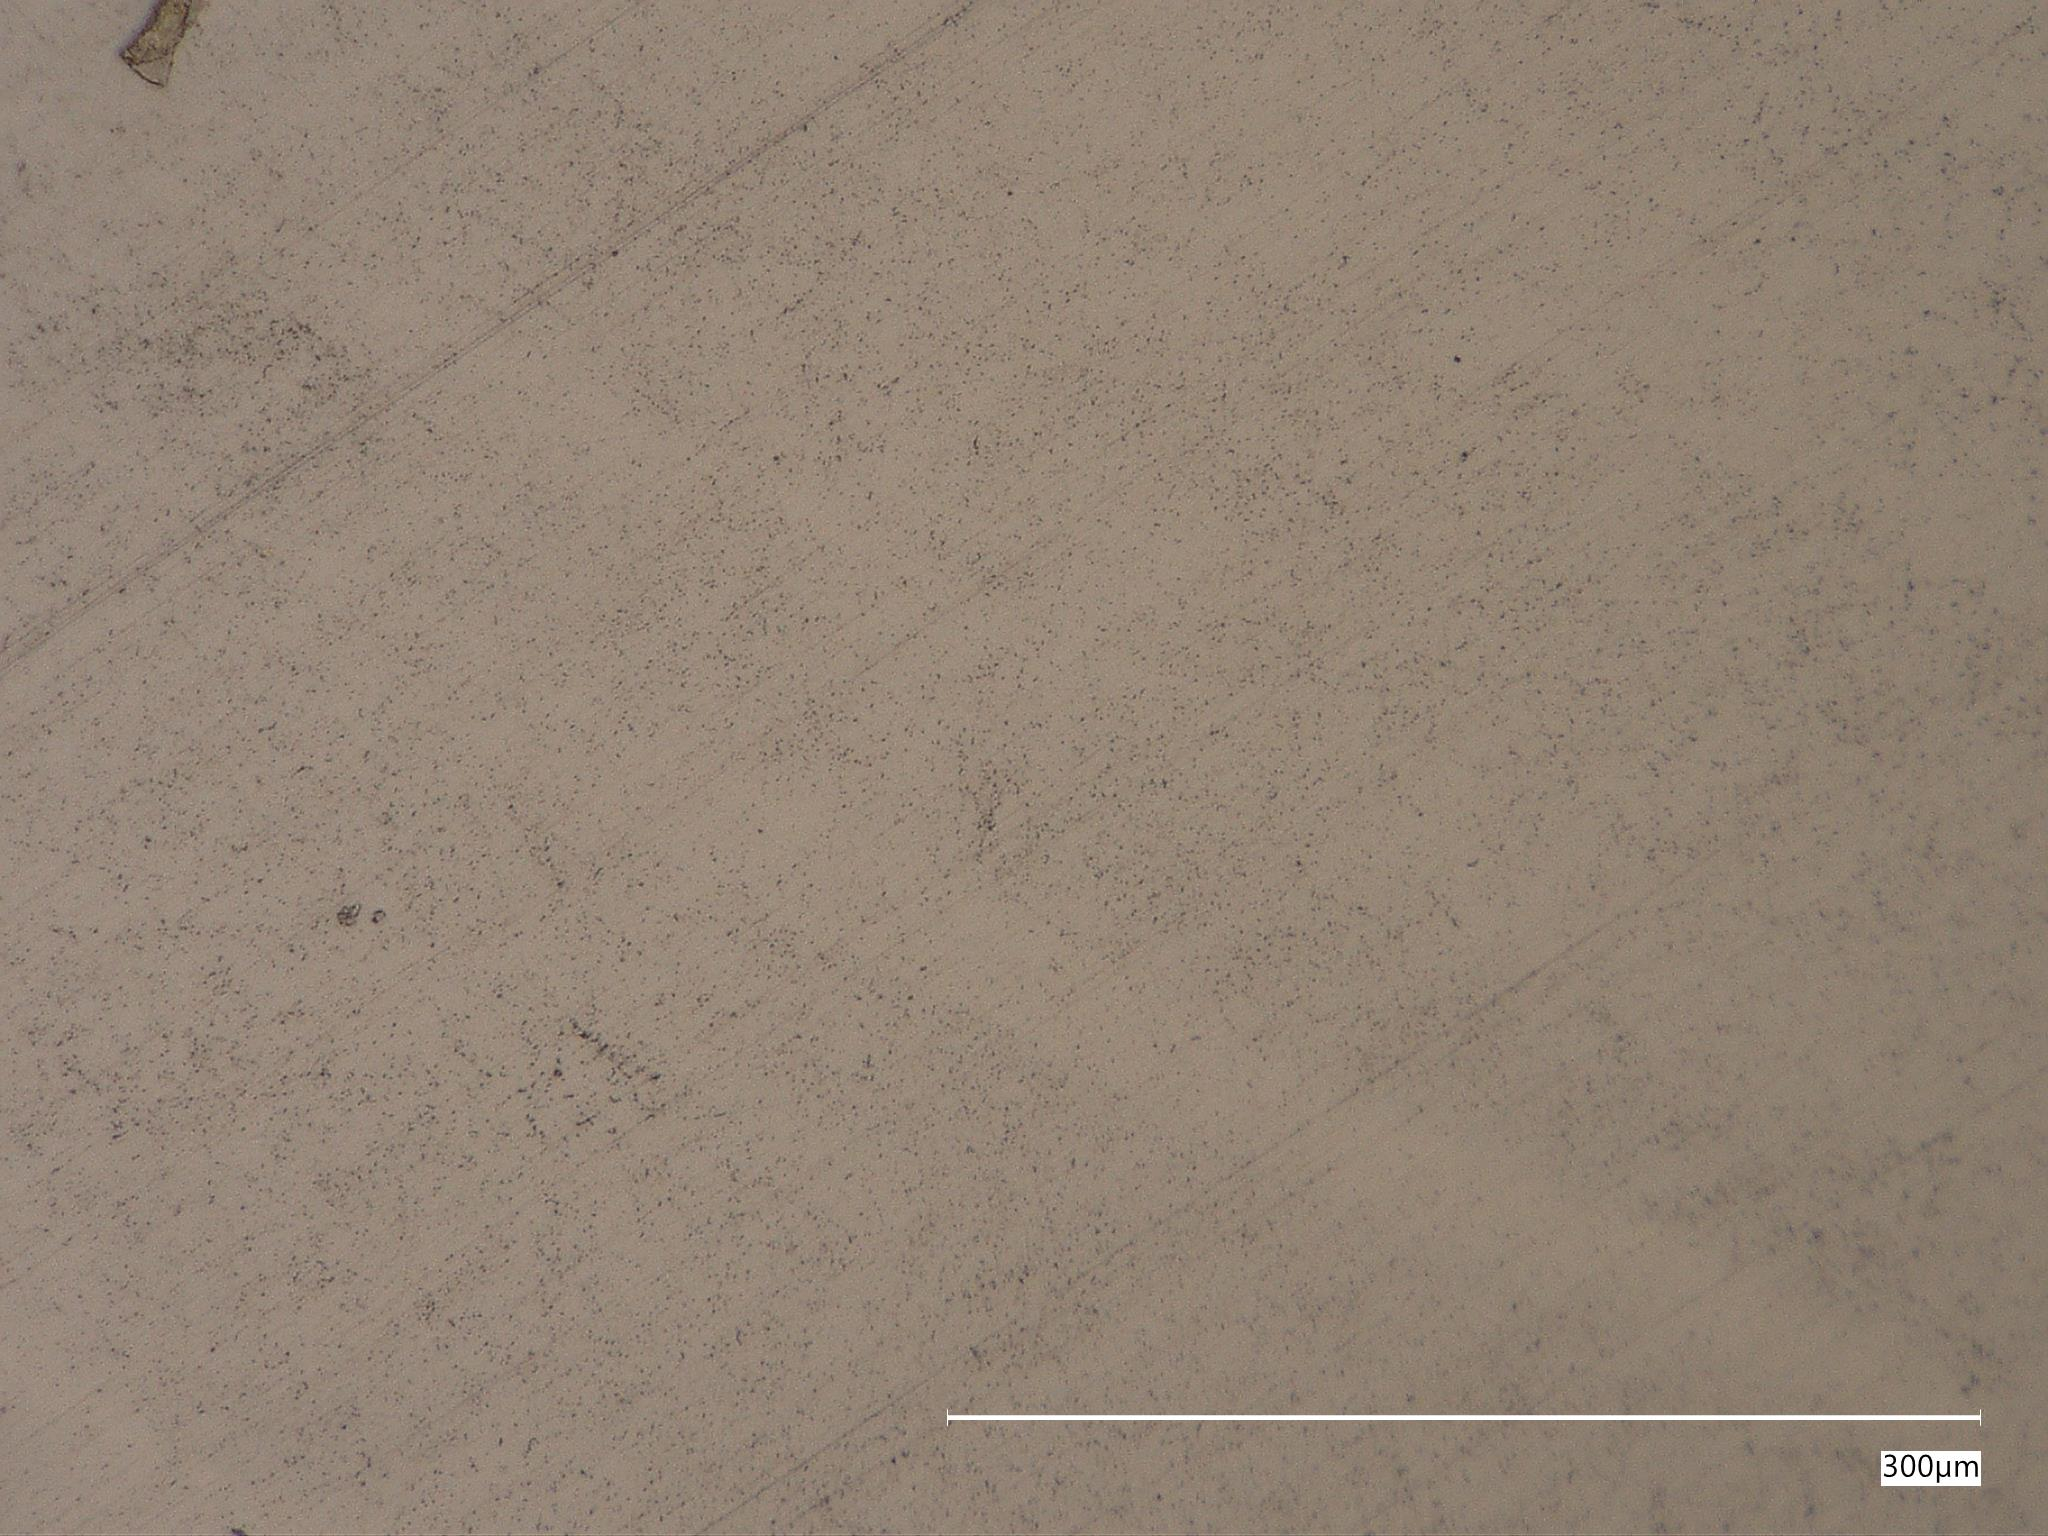
\includegraphics[keepaspectratio, scale=0.07]{fig/241218_304650C2h850C2h_3um.jpg}
      \subcaption{Diamond paste 3$\mu$m}
      \label{fig:8503um}
    \end{minipage}
    \begin{minipage}[htbp]{0.45\linewidth}
      \centering
      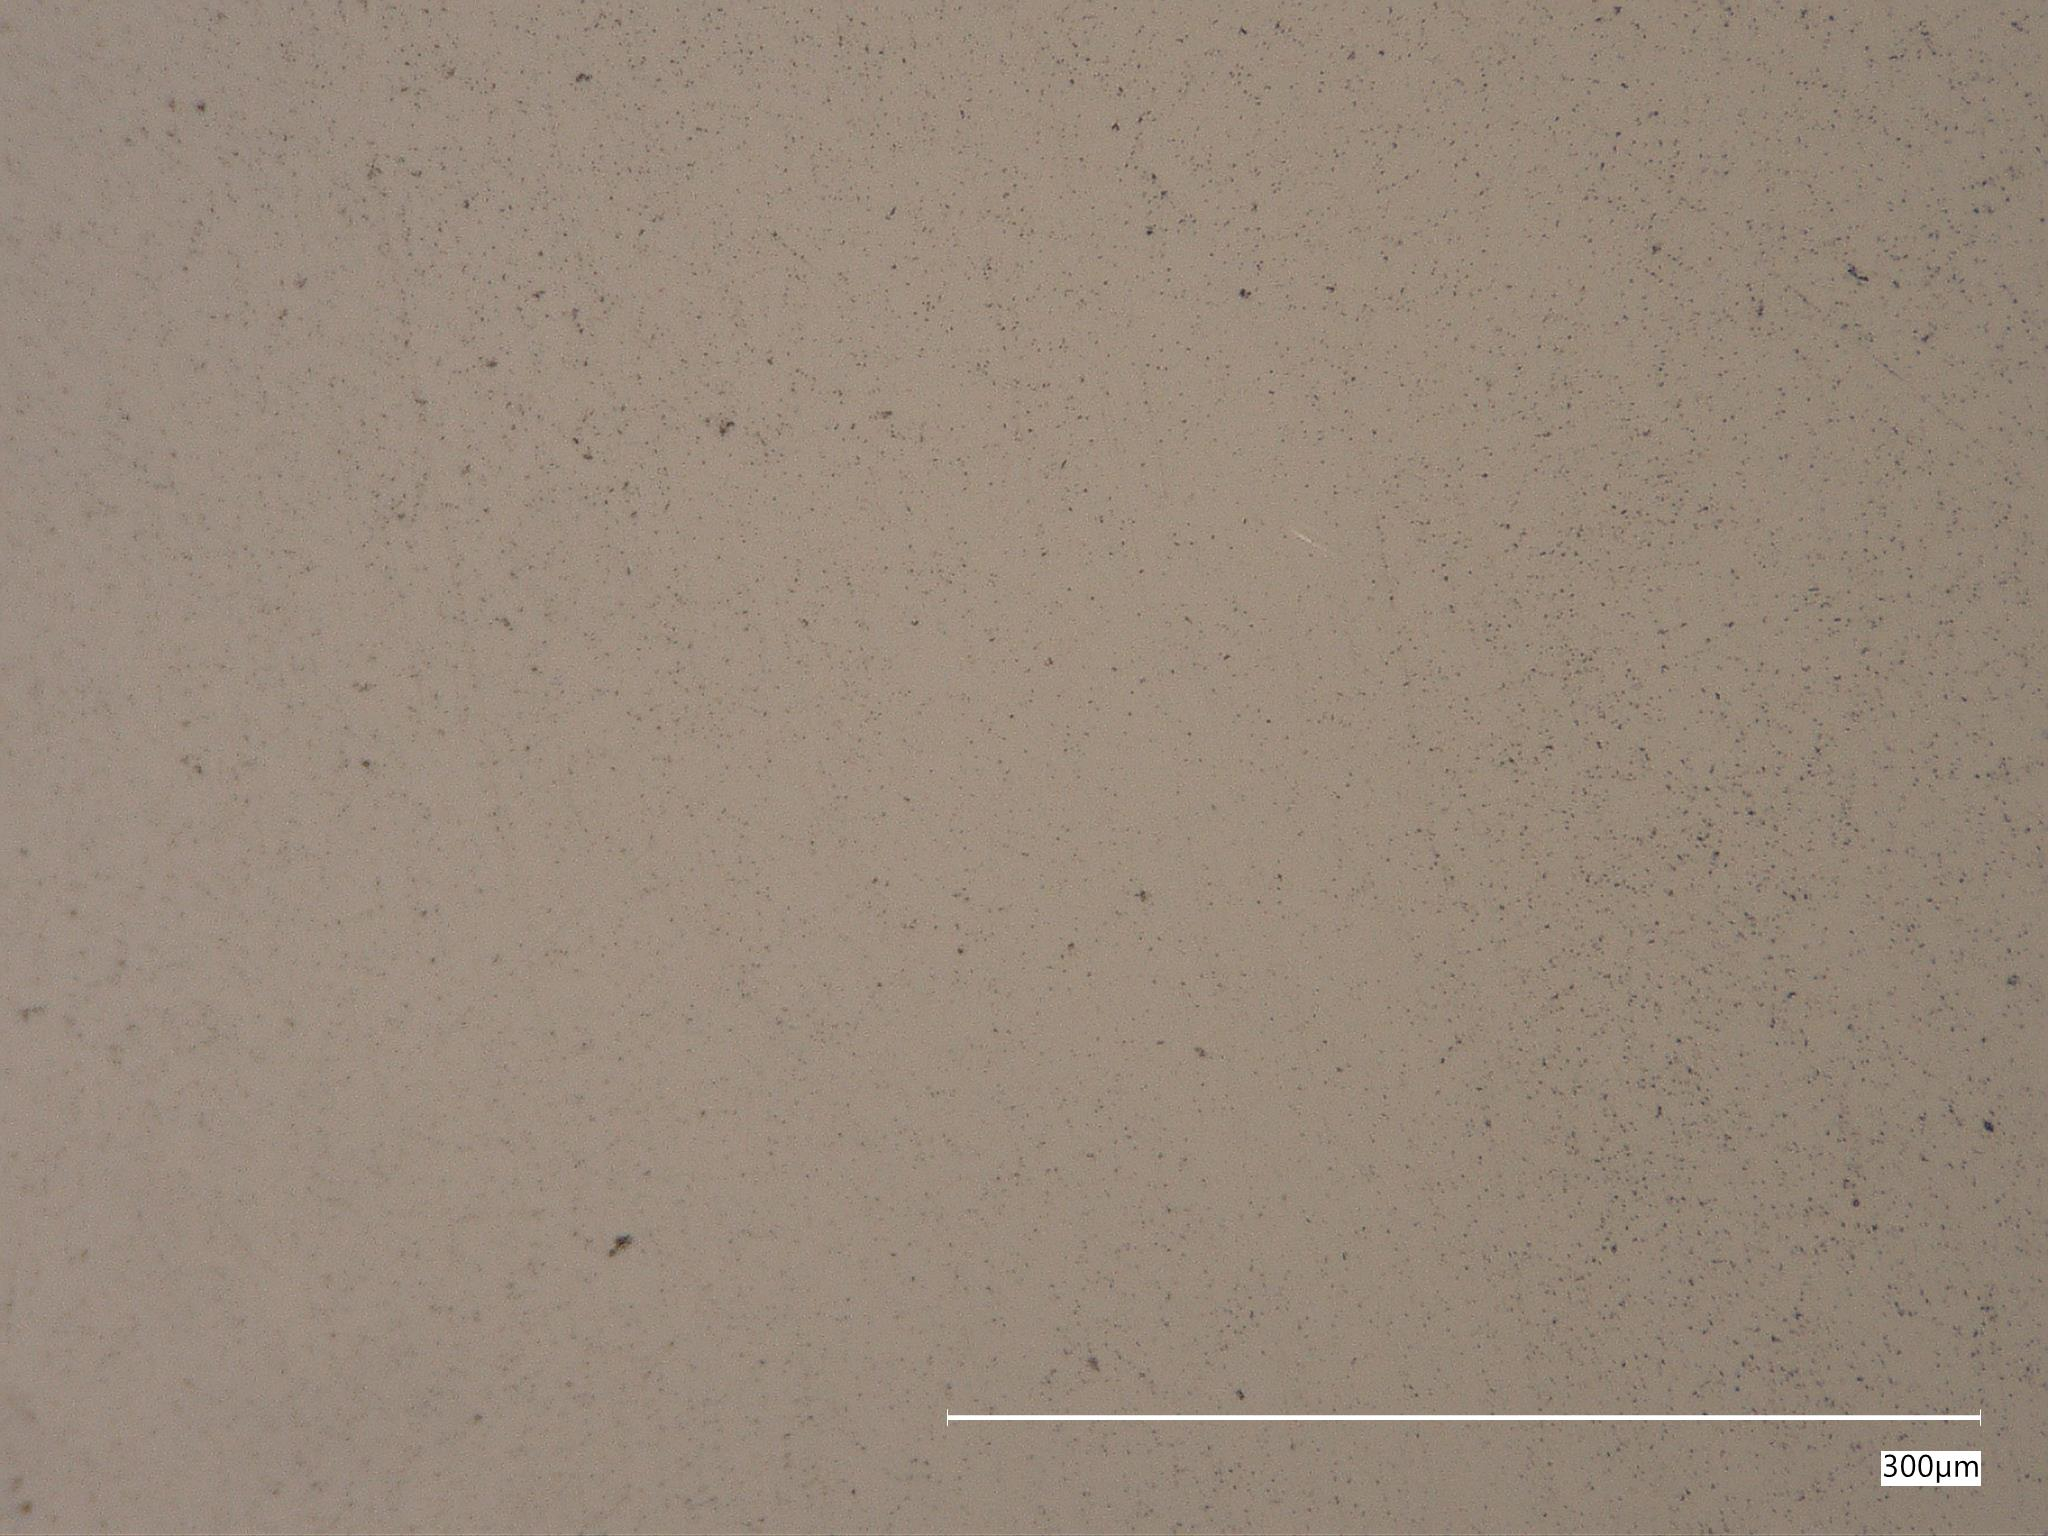
\includegraphics[keepaspectratio, scale=0.07]{fig/241218_304650C2h850C2h_1um.jpg}
      \subcaption{Diamond paste 1$\mu$m}
      \label{fig:8501um}
    \end{minipage}
    \centering
    \caption{SUS304 stainless steel after buffing(650$^\circ$C 2hour + 850$^\circ$C 2hour).}
    \label{fig:304850Buff}
\end{figure}
\begin{figure}[htbp]
    \centering %中央揃え
    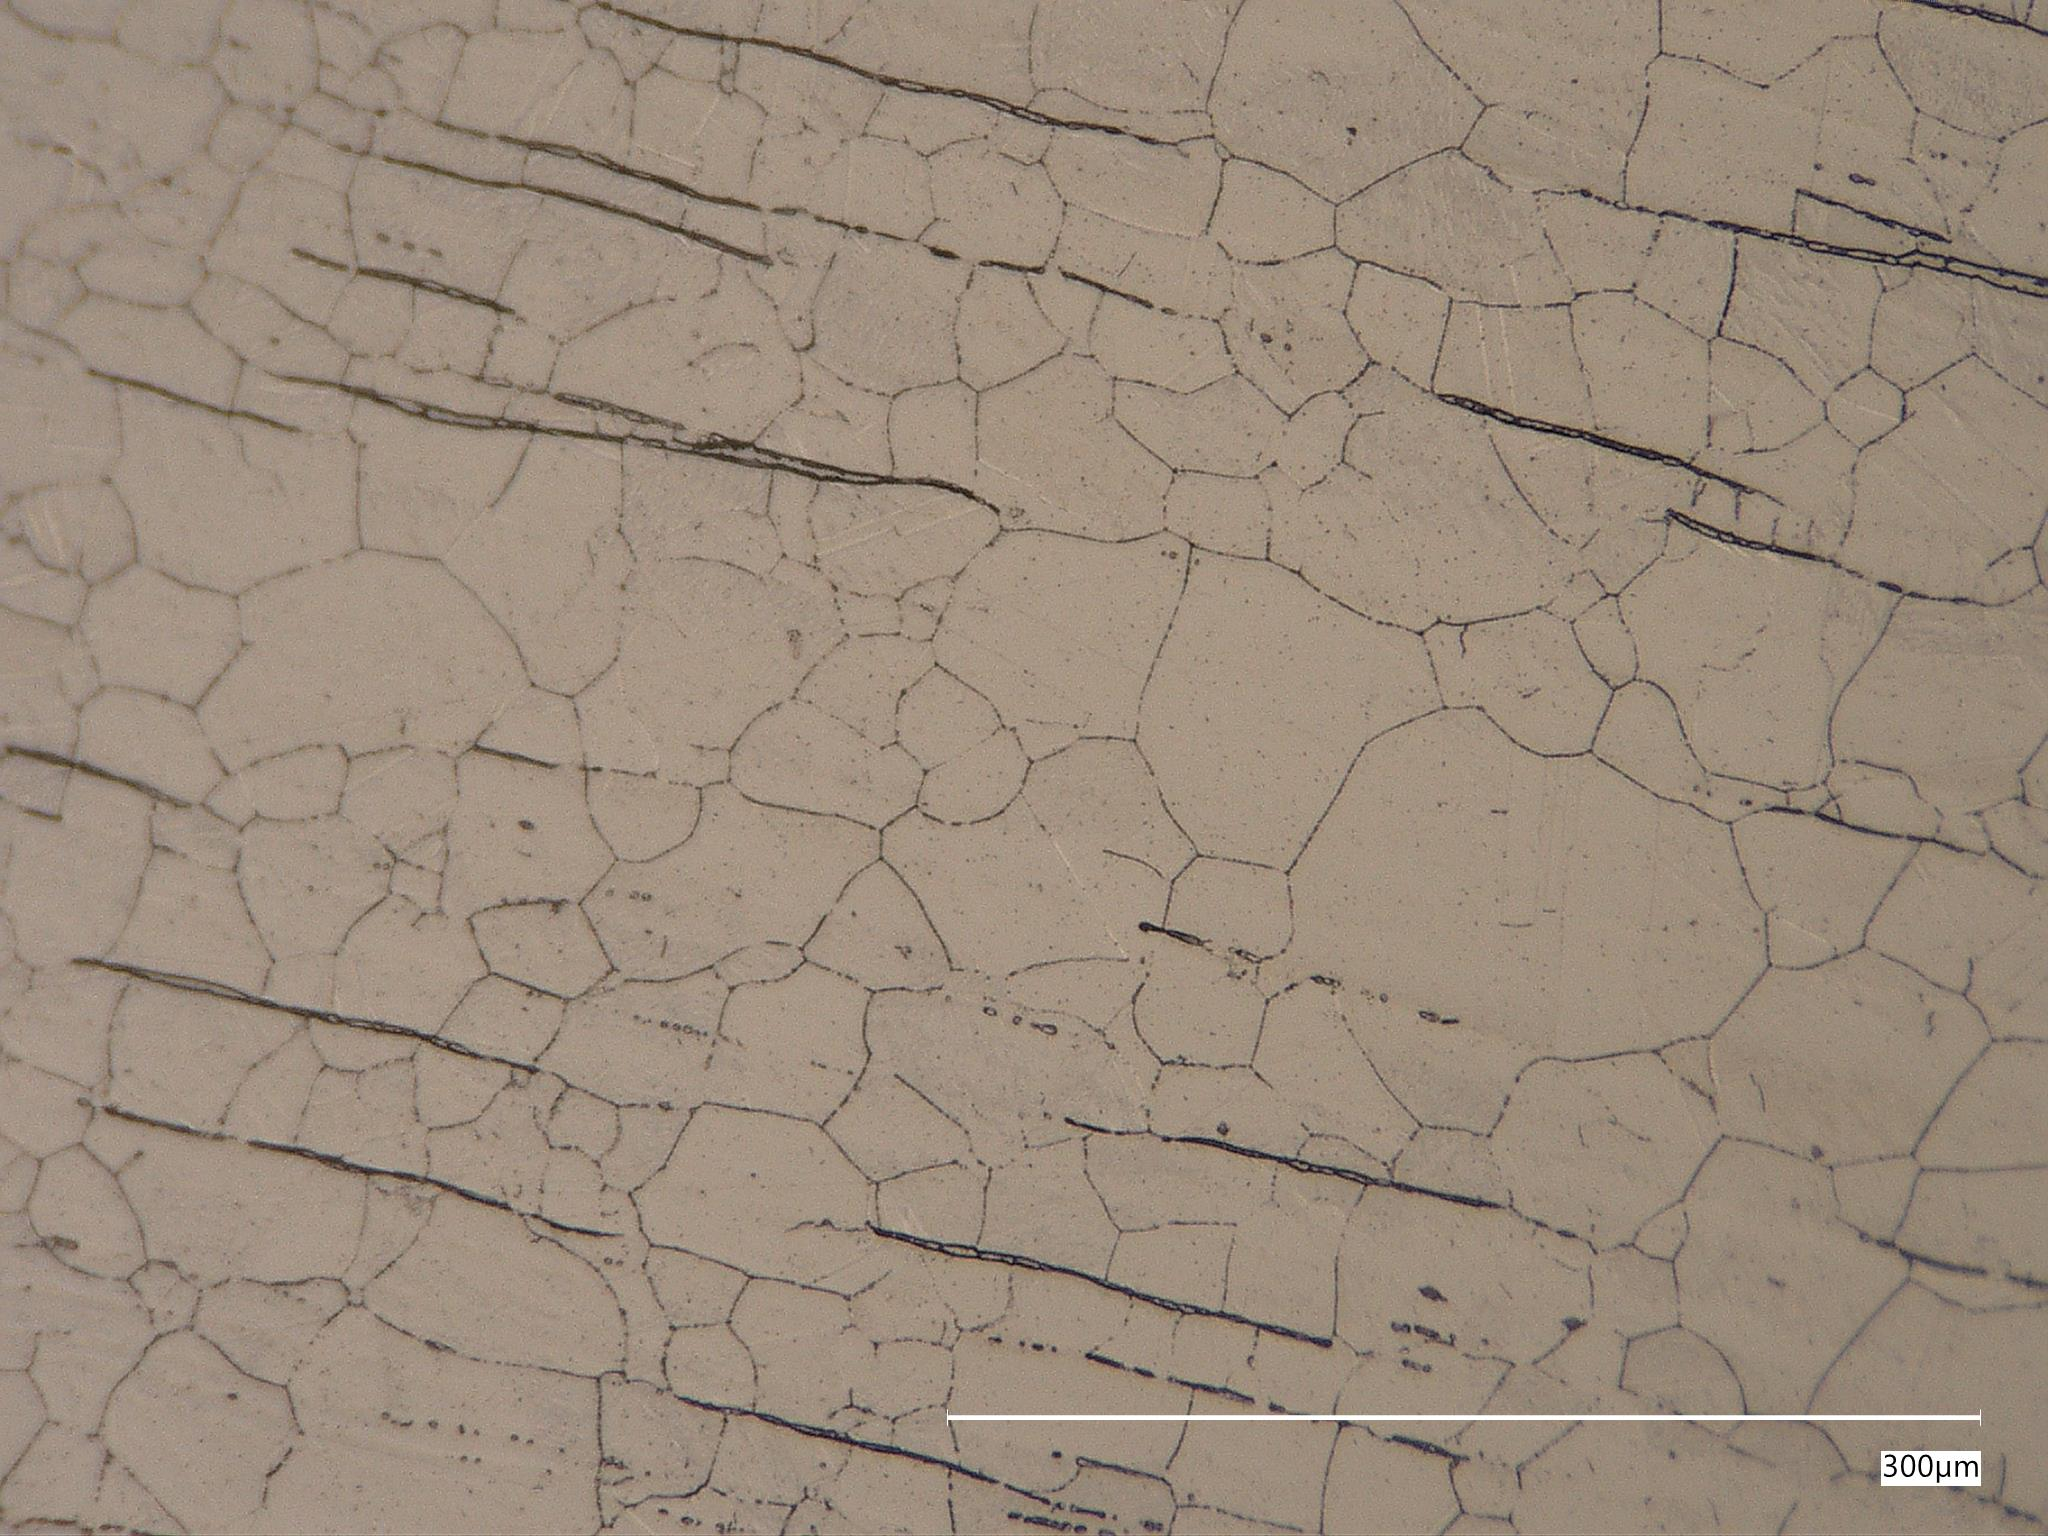
\includegraphics[width=100truemm,clip]{fig/241218_304650C2h850C2h_ethcing.jpg}
    \caption{SUS304 stainless steel after chemical etching(650$^\circ$C 2hour + 850$^\circ$C 2hour).}
    \label{fig:304850Etching}
\end{figure}
\clearpage

図\ref{fig:Cu}に電解研磨する前の銅の表面の撮影結果を示す.図\ref{fig:Cuele}に電解研磨後の銅の表面の撮影結果を示す.電解研磨前の銅の表面には,長い傷が多く存在している.電解研磨後の銅の表面は,平滑化されており傷がなくなっている.丸い点々とした模様があるが,これは電解研磨中に生じた気泡によるものであると考えられる.
\begin{figure}[htbp]
    \centering %中央揃え
    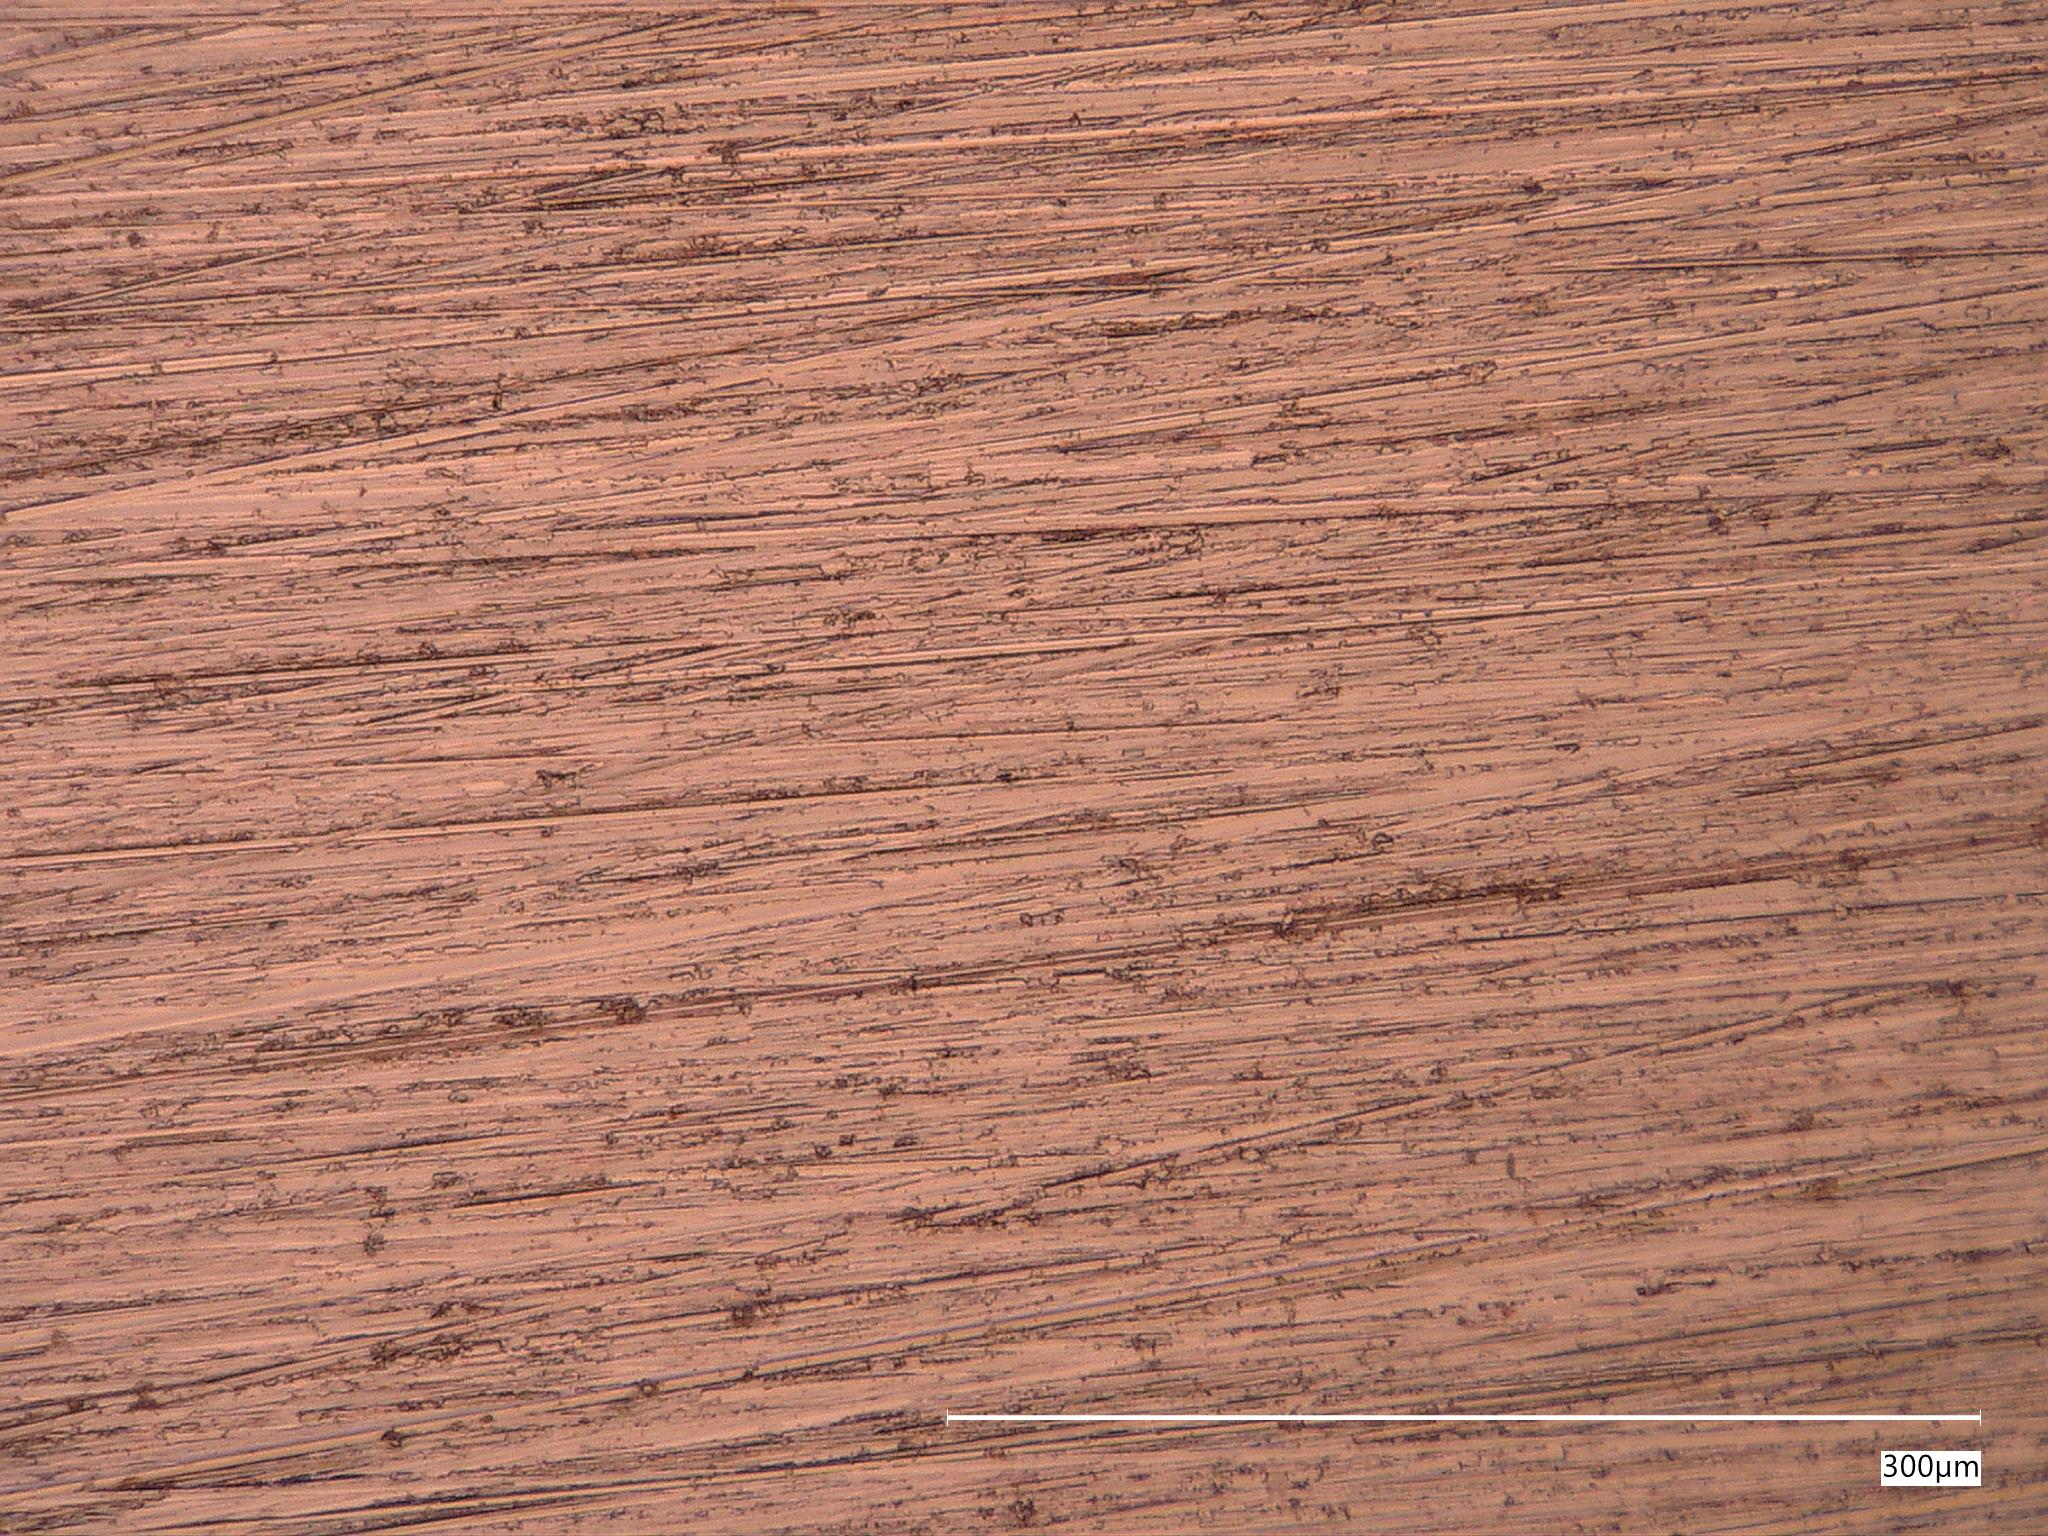
\includegraphics[width=100truemm,clip]{fig/241218_Cu_600.jpg}
    \caption{Copper before electropolishing.}
    \label{fig:Cu}
\end{figure}
\begin{figure}[htbp]
    \centering %中央揃え
    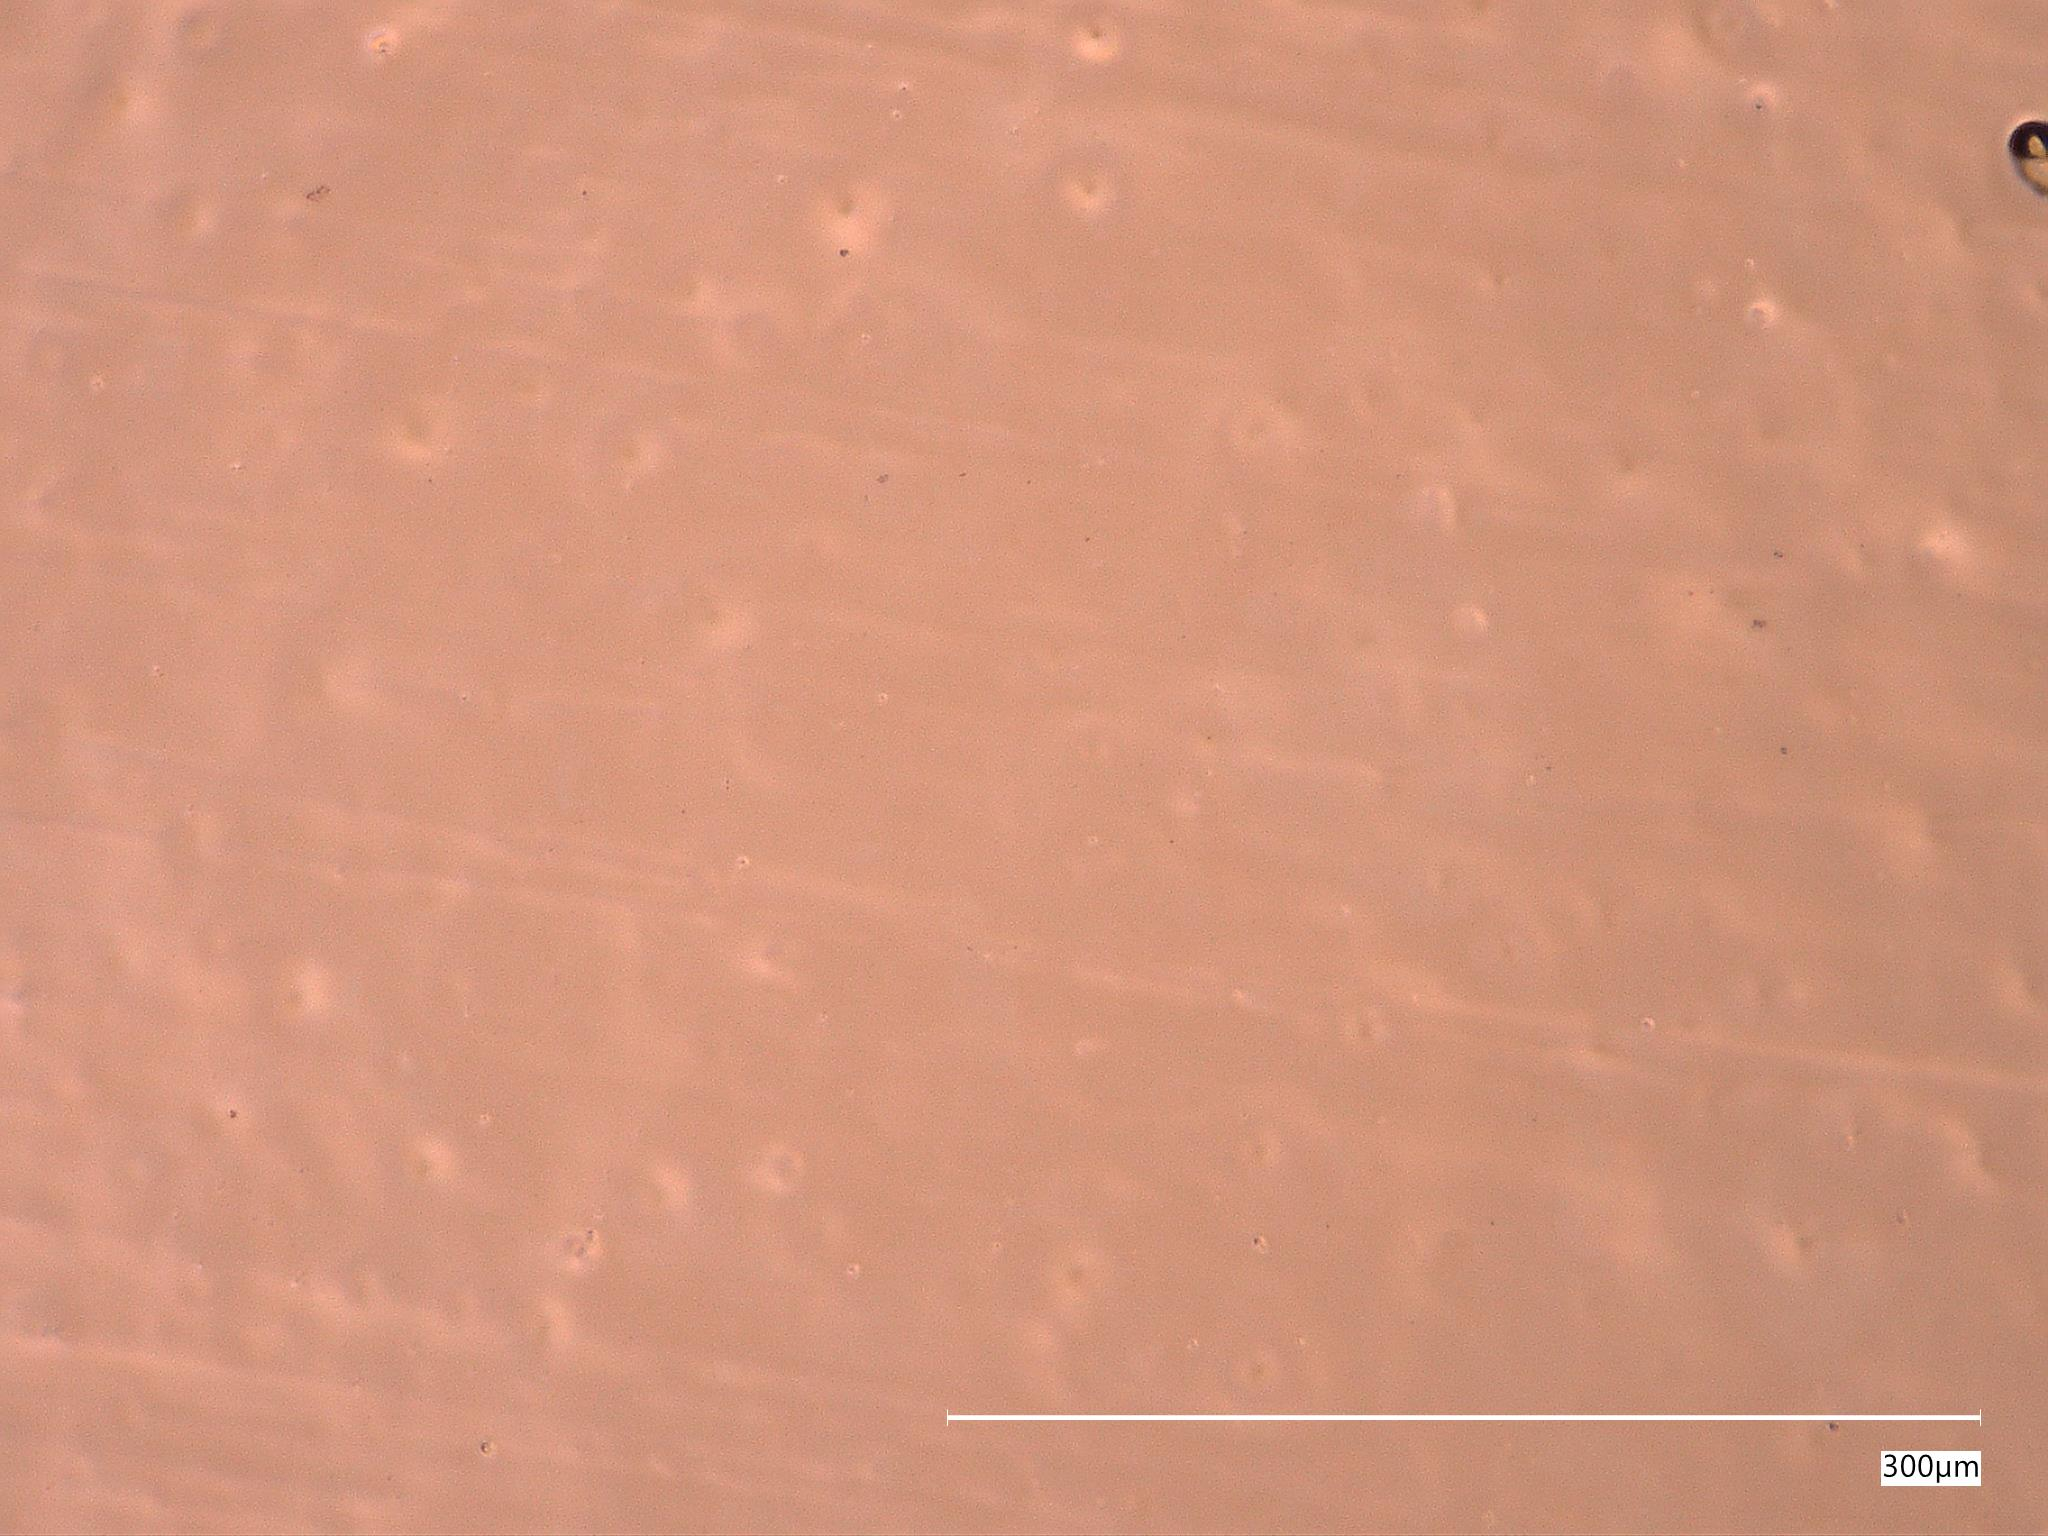
\includegraphics[width=100truemm,clip]{fig/241218_Cu_ele.jpg}
    \caption{Copper after electropolishing.}
    \label{fig:Cuele}
\end{figure}

\clearpage